% ----------------------------------------------------------------------------
% Vorlage Abschlussarbeit Informatik THM (minimal)
%
% Copyright (c) 2016 by Burkhardt Renz. All rights reserved.
% Die Vorlage für eine Abschlussarbeit in der Informatik am Fachbereich
% MNI der THM ist lizenziert unter einer Creative Commons
% Namensnennung-Nicht kommerziell 4.0 International Lizenz.
%
% $Id: vorlage.tex 3835 2016-09-26 09:17:05Z br $
% ----------------------------------------------------------------------------

\documentclass[%
	BCOR=8.25mm,         % Bindekorrektur
	DIV=12,              % Satzspiegel
	parskip=half,				 % Abstand zwischen Absätzen
	bibliography=totoc,	 % Literaturverzeichnis im Inhaltsverzeichnis
	headsepline=on,      % Trennlinie Kolumnentitel
	openany,
	ngerman
	]{scrbook}

%% Präambel
\usepackage[english, ngerman]{babel} % deutsche typogr. Regeln + Trenntabelle
\usepackage[T1]{fontenc}             % interner TeX-Font-Codierung
\usepackage{lmodern}                 % Font Latin Modern
\usepackage[utf8]{inputenc}          % Font-Codierung der Eingabedatei
\usepackage[babel]{csquotes}         % Anführungszeichen
\usepackage[figurename=Abbildung]{caption}
\usepackage{graphicx}                % Graphiken
\usepackage{booktabs}                % Tabellen schöner
\usepackage{listingsutf8}            % Listings mit Einstellungen
\usepackage{chngcntr}
\counterwithout{footnote}{chapter}   % Document Wide cite index
\lstset{basicstyle=\small\ttfamily,
	tabsize=2,
	basewidth={0.5em,0.45em},
	extendedchars=true}
\usepackage{amsmath}	            % Mathematik
\usepackage{enumitem}				% Listen Aufzählung
\usepackage[section]{placeins}
\makeatletter						% Expand placeins function to subsection
\AtBeginDocument{%
	\expandafter\renewcommand\expandafter\subsection\expandafter{%
		\expandafter\@fb@secFB\subsection
	}%
}
\makeatother
\usepackage{geometry}
%\geometry{a4paper
%	,left=40mm, right=15mm, top=20mm, bottom=15mm   %Seitenr"ander
	%,body={11cm,17cm}
	%,textheight=17cm,textwidth=11cm
%	,headsep=1cm      %Abstand Seitenzahl - Text
%	,showframe=true
%}
\usepackage[english]{babel}
\usepackage[backend=biber,maxnames=999,style=alphabetic]{biblatex}
\addbibresource{bib/library.bib} 
\usepackage{scrhack}								 % unterdrückt Fehlermeldung von listings
%% Nummerierungstiefen
\setcounter{tocdepth}{2}             % 3 Stufen im Inhaltsverzeichnis
\setcounter{secnumdepth}{3} 		     % 3 Stufen in Abschnittnummerierung


 
%% Literaturverzeichniss Format
% Adapted from \footcite in numeric.cbx and generic citation
% commands \citeauthor, \citetitle, \citeyear in biblatex.def
\DeclareCiteCommand{\footpartcite}[\mkbibfootnote]
{\usebibmacro{prenote}}
{\usebibmacro{citeindex}%
	\mkbibbrackets{\usebibmacro{cite}}%
	\setunit{\addnbspace}
	\printfield[citetitle]{title}%
	\newunit
	\printfield{year}
}
{\addsemicolon\space}
{\usebibmacro{postnote}}

\DeclareMultiCiteCommand{\footpartcites}[\mkbibfootnote]{\footpartcite}{\addsemicolon\space}

%% Römische Nummer im Textverweden
\newcommand{\uproman}[1]{\uppercase\expandafter{\romannumeral#1}}
\newcommand{\lowroman}[1]{\romannumeral#1\relax}


%% Chapterschriftformatierung
\usepackage{titlesec, blindtext, color}
\definecolor{gray75}{gray}{0.75}
\newcommand{\hsp}{\hspace{20pt}}
\titleformat{\chapter}[hang]{\Huge\bfseries}{\thechapter\hsp\textcolor{gray75}{|}\hsp}{0pt}{\Huge\bfseries}

\usepackage[pdftex]{hyperref}       
\hypersetup{
	bookmarksopen=true,
	bookmarksopenlevel=3,
	colorlinks,
	citecolor=blue,
	linkcolor=blue,
}
\usepackage{cleveref}               % Smart Cross-Doc refs
\urlstyle{same}  % don't use monospace font for urls
%% Glossardefinition
\usepackage{subcaption} % Images horizontially
\usepackage[toc,acronym]{glossaries} % Glossarpaket
\makeglossaries
\renewcommand*{\acronymname}{Abkürzungsverzeichnis}
\newglossaryentry{latex}
{
	name={latex},
	description={Is a mark up language specially suited for scientific documents}
}

\newacronym{fpsLabel}{FPS}{Frames per Second}
\newacronym{MMULabel}{MMU}{Memory Mangagment Unit}
\newacronym{cpuLabel}{CPU}{Central Processor Unit}
\newacronym{gpuLabel}{GPU}{Graphical Processor Unit}
\newacronym{ramLabel}{RAM}{Random-Access Memory}
\newacronym{hddLabel}{HDD}{Hard Disk Drive}
\newacronym{tcpLabel}{TCP}{Transmission Control Protocol}
\newacronym{ipLabel}{IP}{Internet Protocol}
\newacronym{httpLabel}{HTTP}{Hypertext Transfer Protocol}
\newacronym{iotLabel}{IoT}{Internet of Things}
\newacronym{apiLabel}{API}{Application Programming Interface}
\newglossaryentry{cpuGlossar}{
	name={Zentrale Verarbeitungseinheit},
	description={Die zentrale Verarbeitungseinheit, im englischen auch \emph{Central Processor Unit} (CPU) genannt, ist die Komponente eines Systems, welches für die Abarbeitung des Maschinenprogramms zuständig ist. Im Allgemeinen Sprachgebraucht umfasst der Begriff der CPU mehrere Teilkomponenten, wie zum Beispiel dem Steuerwerk, der Register, des Speichermanagers (\gls{MMULabel})}}
\newglossaryentry{ciGlossar}{
	name={Continues Integration},
	description={Automatisierter und fortlaufend getätigter Integrationsprozess von Änderungen einer Anwendungen.}}
\newglossaryentry{renderingGlossar}{
	name={Rendering},
	description={
	Rendering ist das erzeugen von zwei-dimensionalen Bildern.
	Rohdaten, wie z.B. virtuelle Kameras, drei-dimensionale Objekte, Lichtquellen, etc. werden dazu genutzt, um diese Bilder zu generieren}
}

\pagenumbering{roman}
% ----------------------------------------------------------------------------
\begin{document}
\frontmatter

%% Titelseite
\begin{titlepage}
	\begin{center}
	
\includegraphics[width=0.9\textwidth]{img/mni-logo}\\[5cm]
	\textbf{\huge\sffamily Generierung und Ordnung von Events in verteilten Systemen mit asynchroner Kommmunikation}\\[2cm]
	\textsc{\Large Bachlorthesis}\\Studiengang Informatik\\[2cm]
	vorgelegt von\\
	\textbf{Simon Stockhause}\\ [1.5cm] 
	Mai 2020
	\end{center}
	\vfill
	\center
	\begin{tabular}{ll}
		Referent der Arbeit: & Prof. Dr. Harald Ritz\\ 
		Korreferent der Arbeit: & M.Sc. Pascal Bormann\\ 
	\end{tabular}
\end{titlepage}
\cleardoubleemptypage

%% Erklärung
\pagestyle{empty}
{
	\renewcommand{\thispagestyle}[1]{}
 Hier Steht Erklärung
}
\clearpage
\pagestyle{plain}

%% Zusammenfassung
\pagestyle{empty}
\begin{quote}
	\vspace*{4cm}

	\begin{center}
		\textbf{\Large\sffamily Zusammenfassung}
	\end{center}
\end{quote}
\cleardoubleemptypage

%% Verzeichnissse
%% Kommando sorgt für das Entfernen der Seitennummerierung in römischen Zahlen 
%% bei Inhaltsverzeichniss und Abbildnugsverzeichniss

\pagestyle{empty}
{
	\renewcommand{\thispagestyle}[1]{}
	\tableofcontents
}
\clearpage
\pagestyle{plain}
\pagestyle{empty}
{
	\renewcommand{\thispagestyle}[1]{}
	\listoffigures
}
\clearpage
\pagestyle{plain}

\mainmatter 
\pagestyle{headings}

\pagenumbering{arabic}
% ----------------------------------------------------------------------------
% Copyright (c) 2016 by Burkhardt Renz. All rights reserved.
% Die Vorlage für eine Abschlussarbeit in der Informatik am Fachbereich
% MNI der THM ist lizenziert unter einer Creative Commons
% Namensnennung-Nicht kommerziell 4.0 International Lizenz.
%
% Id:$
% ----------------------------------------------------------------------------

\chapter{Einleitung}

\section{Motivation}
\section{Problemstellung}
\section{Foschungsstand}
\section{Thesisübersicht}
% ----------------------------------------------------------------------------

% ----------------------------------------------------------------------------
% Copyright (c) 2016 by Burkhardt Renz. All rights reserved.
% Die Vorlage für eine Abschlussarbeit in der Informatik am Fachbereich
% MNI der THM ist lizenziert unter einer Creative Commons
% Namensnennung-Nicht kommerziell 4.0 International Lizenz.
%
% Id:$
% ----------------------------------------------------------------------------

\chapter{Themenüberblick}

\section{Verteilte Systeme}
\subsection{Überwachung von verteilten Systemen}
\subsection{Synchronisation}
\subsection{Ordnung von events}
\section{Bibliotheksentwicklung}
% ----------------------------------------------------------------------------

% ----------------------------------------------------------------------------
% Copyright (c) 2016 by Burkhardt Renz. All rights reserved.
% Die Vorlage für eine Abschlussarbeit in der Informatik am Fachbereich
% MNI der THM ist lizenziert unter einer Creative Commons
% Namensnennung-Nicht kommerziell 4.0 International Lizenz.
%
% Id:$
% ----------------------------------------------------------------------------

\chapter{Problembeschreibung}
\label{chapter:Problembeschreibung}
In diesem Kapitel wird die Problematik, um das Generieren und Ordnen von Events in einem verteilten System mit asynchroner Kommunikation, beschrieben. Dabei betrachten man die Relevanz der Problemstellung. Ausserdem werden Fragen aufgestellt, die diese Problemstellung umfassen. Anschließend wird eine Anforderungsanalyse durchgeführt.

\section{Anwendungsüberwachung}
\label{section:Tracing von Anwendungen}
Viele Bereiche der Wirtschschaft, der Wisschenschaft und grundsätzlich des alltäglichen Lebens sind Software unterstützt. Trends wie beispielsweise \gls{iotLabel}, Hausautomatisierung, Mobile Geräte, etc. sind Anwendungsbeispiele. Diese sind aus ihrer Natur heraus stark verteilte Anwendungen. Aber auch potentiell neue Anwendungsbereiche, wie zum Beispiel verteiltes \gls{renderingGlossar}, benötigen detailierte Einsicht in die internen Vorgänge der Anwendung. 

Dabei spielen zwei Eigenschaften in der Überwachung der Anwendung eine zentrale Rolle. 
Zum einen ist das die (\lowroman{1}) \emph{Performance} und zum anderen die (\lowroman{2}) \emph{Korrektheit}.


\textbf{Performance} \space\space\space 
Viele Anwendungsbereiche setzten gewisse Rahmenbedingungen, die erfüllt werden müssen. 
Nutzererwartungen im Bezug auf interaktive Systeme, welches einer der beiden Anwendungsfälle der Instrumentalisierungsbibliothek ist, äußern sich beispielsweise in der Reaktionszeit der Anwendung auf Benutzereingaben. 
Das Rendering nimmt dabei nur einen Teil der Gesamtlatenz ein.
Ein beispielhafter Gesamtpfad, der durch die verteilte Renderinganwendung genommen werden kann, besteht aus dem Senden der Benutzereingabe, der Übermittlung der Benutzereingabe zum verteilten System, der Verarbeitung der Eingabe und der Übermittlung des Ergebnisses an die Benutzeranwendung.
\cref{fig:Anwendungsueberwachung_Gesamtsystem} verdeutlicht diesen Pfad von kausal relatierenden Events.
Dabei ist jede Komponente des Pfades ein generiertes Event.
Zu sehen ist, dass das (1) Senden der Benutzereingabe vor dem (2) Übermitteln der Benutzereingabe stattfinden.
Anschließend wird die Eingabe (3) Empfangen.
Auch die (4) Verarbeitung im verteilten System, das für den Benutzer, wie in \cref{subsection:Eigenschaften eines verteilten Systems} definiert, nicht als solches kenntlich sein muss, generiert in diesem Beispiel ein Event.
Die Antwort wird (5) gesendet und die (6) Übermittlung wird durchgeführt.
Zuletzt wird die Antwort (7) empfangen. Das Empfangen schließt den Pfad ab. Die Gesamtdauer des Pfades wird als Latenz eines Frames bezeichnet.
Daraus kann eine Durschschnittslatenz über eine Zeitspanne berechnet werden, welches als Performanceindikator dient. Die Zeitspanne zwischen den einzelnen Events können verglichen werden. Dabei ist es möglich sog. \emph{Bottlenecks} zu identifizieren. Bottlnecks sind Vorgänge, die einen großteil der Gesamtdauer ausmachen. Sind werden durch die Zeitspanne zwischen zwei Events, die auf dem \emph{kritischen Pfad} liegen, bestimmt. Diese Art der Anwendungsüberwachung soll die Möglichkeit bieten, Bottlenecks zu identifizieren. Wie in \cref{subsection:Ordnung von Events} beschrieben, verlangt eine Messung der Zeit über verschiedene physikalisch Entitäten entweder eine globale physikalische Uhr oder jeweils eine physikalische Uhr in jeder Entität, die über alle Entitäten synchrone sind beziehungsweise, synchronisiert werden. Dabei stellt sich die Frage, \emph{inwiefern eine solche Zeitmessung von Zeitspannen zwischen Events konzipiert werden kann. } 


\begin{figure}[!ht]
	\centering
	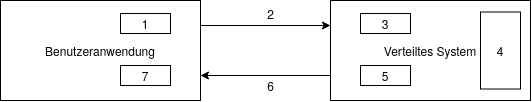
\includegraphics[scale=0.5]{img/Problembeschreibung/Anwendungsueberwachung_Gesamtsystem.png}
	\caption[Kausaler Pfad einer Vorgangs in dem verteilten rendering System]{Kausaler Pfad einer Vorgangs in dem verteilten rendering System}
	\label{fig:Anwendungsueberwachung_Gesamtsystem}
\end{figure}

\textbf{Korrektheit} \space\space\space Die Korrektheit eines Systems ist dann gegeben, wenn die Eigenschaften eines Systems einer \emph{Spezifikation} entsprechen. Das bedeutet, dass die Beobachtung des Verhaltens einer (verteilten) Anwendung nicht ausreicht, um seine Korrektheit zu beweisen. Tracing soll also nicht die Korrektheit einer verteilten Anwendung beweisen. Tracing kann aber dabei unterstützen, indem es das Verhalten einer Anwendung beobachtbar macht. Insbesondere die Zusammenhänge der Komponenten und die entstehenden Nebenläufigkeiten sind erschwerende Faktoren in der Verifikation. So stellt sich die Frage, ob \emph{kausal zusammenhängende Events derart dargestellt werden können, dass anhand einer Visualisierung feststellbar ist, ob das Verhalten der Anwendung starke Ausreißer, die auf Fehlimplmenentierung deuten könnten, aufweist.}


\section{Zusammenführung von Events}
\label{section: Ordnungsproblem von Events}
\begin{figure}[!ht]
	\centering
	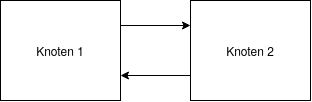
\includegraphics[scale=0.5]{img/Problembeschreibung/distributed_system_application_minimal.png}
	\caption[Minimale Struktur eines verteilten Systems]{Minimale Struktur eines verteilten Systems, bestehend aus zwei Komponenten}
	\label{fig:distributed_system_application_minimal}
\end{figure}
\begin{figure}[!ht]
	\centering
	\begin{subfigure}[t]{.49\linewidth}
		\centering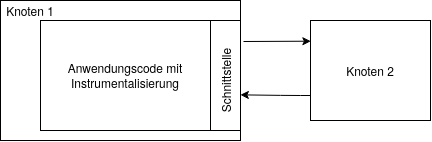
\includegraphics[width=0.9\linewidth]{img/Problembeschreibung/distributed_system_application_inside.png}
		\caption[Abbildung]{zeigt Knoten mit instrumentalisiertem Anwendungscode}
		\label{fig:distributed_system_application_inside}
	\end{subfigure}
	\begin{subfigure}[t]{.49\linewidth}
		\centering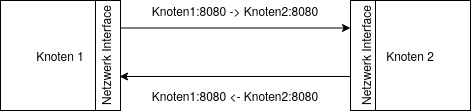
\includegraphics[width=\linewidth]{img/Problembeschreibung/distributed_system_network.png}
		\caption[Abbildung]{Netzwerkkommunikation über TCP/IP}
		\label{fig:distributed_system_network}
	\end{subfigure}
	\caption[Anwendungsinstrumentalisierung und Netzwerkkommunikation über TCP/IP in verteilten Systemen]{}
\end{figure} 

Man definieren ein minimales verteiltes System, welches das verteilte rendering System vereinfacht darstellt. Dieses besteht aus zwei Komponenten. \cref{fig:distributed_system_application_minimal} bildet ein solches System ab. Die Knoten beinhalten zwei für das Generieren und Ordnen von Events interessante Aspekte. Dies ist zum einen die in \cref{fig:distributed_system_application_inside} dargestellte verteilte Anwendung mit ihrem instrumentalisiertem Code und zum anderen das in \cref{fig:distributed_system_network} dargestellte Netzwerk, über welches Nachrichten ausgetauscht werden. 

 \begin{figure}[!ht]
	\centering
	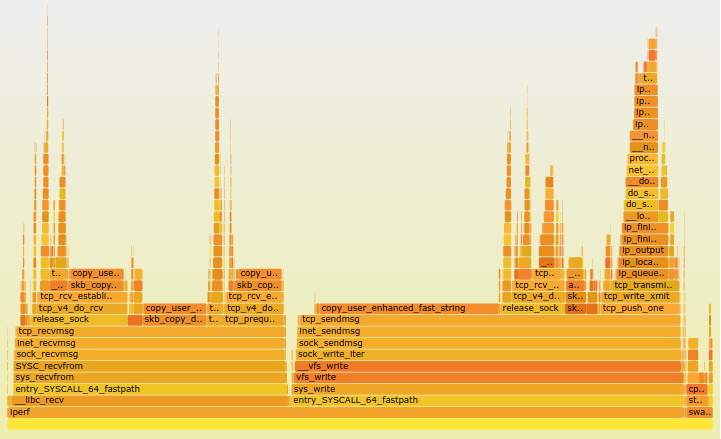
\includegraphics[scale=0.5]{img/Problembeschreibung/problembeschreibung_flamengraph.png}
	\caption[Visualisierung von CPU Performancedaten]{Visualisierung von CPU Performancedaten dargestellt als Flammengraph von Brendan D. Gregg \cite{BrendanGregg2011}}
	\label{fig:problembeschreibung_flamengraph}
\end{figure}

Die Komponenten des Systems besitzen jeweils einen Linux Kernel. Der Kernel bietet die Funktionalität \emph{perf\_events} zu erheben. 
\begin{quote}
	perf\_events ist ein eventorientiertes Überwachungswerkzeug, welches helfen kann, Leistung zu verbessern und Fehelerquellen von Funktionen zu lokalisieren. 
	\footpartcite{BrendanGreggPerf}
\end{quote}
Von dem Szenario ausgehend, dass man Events innerhalb des Minimalbeispiels analysieren möchte, eignen sich Flammengraphen.
 Der in \cref{fig:problembeschreibung_flamengraph} gezeigte Flammengraphe stellt perf\_events dar, die während einer TCP Kommunikation erhoben worden sind.  Dabei ist die Länge der Balken, die Zeit, die das Event, relativ zur Gesamtzeit der Messung, insgesamt eingenommen hat. Die erhobenen perf\_event Daten sind Stichproben. Man geht in diesem Beispiel allerdings davon aus, das alle Events aufgenommen worden sind. Diese Darstellung erlaubt es, die Events \emph{eines} Systems genau zu beschreiben. Nun kommt das zweite System hinzu, mit dem die Kommunikation stattgefunden hat. Auch hier sei gegeben, dass das zweite System Daten generiert hat, welche zu einer ähnlich aufgebaute Visualisierung führt. Die beiden Flammengraphen werden miteinandener verbunden. Dies führt zu einer dreidimensionalen Darstellung von Flammengraphen, gezeigt in \cref{fig:flamegraph_3D}. Wie in einer TCP-Verbindung üblich, wird eine Kommunikationskanal aufgebaut. Über den Kanal können Nachrichten ausgetauscht werden. Anschließend wird die Verbindung mit einem Vier-Wege-Handschlag beendet. Die obersten Blöcke und ihre systemübergreifenden Verbindungslinien, dargetellt durch die gestrichelten Linien mit Pfeilrichtung, stellen die Terminierung der TCP-Verbindung dar.
 
 Der Terminierungsprozess wird genauer betrachtet. \cref{fig:flamegraph_3D_closing} zeigt vier Events. \textbf{A} ist die \emph{FIN} Markierung des Initiators. Sie leitet die Terminierung ein. \textbf{C} stellt das Empfangen und Beantworten mittels \emph{ACK} und \emph{FIN} dar. \\
 \textbf{B} ist der Terminierungsmoment des Initatorsystems. Dieser findet nach dem Zeitpunkt des Eintreffens von \emph{FIN} des Empfänger statt. Dieser Zeitpunkt ist das Senden des letzten \emph{ACK} des Initators, addiert mit einer Konstante \emph{Timeout}.  Event \textbf{B} ist also definiert als:
 
\[
	\text{B}: \; Ack_{init} + Timeout  
\]

 \textbf{D} ist der Terminierungsmoment des Empfängersystems. Dieser Zeitpunkt ist das Erhalten der letzten, vom Initiatorsystem gesendeten, \emph{ACK} Makierung. Die unbekannte Variable \emph{Übertragungszeit} nimmt Einfluss auf den Zeitpunkt. Event \textbf{D} ist also definiert als:
 \[
 \text{D}: \; Ack_{init} + Übertragungszeit 
 \]
 
 Zu untersuchen sind die Relationen zwischen diesen vier Events.
 Dabei sind zwei Relationen, wie in \cref{subsection:Ordnung von Events} beschrieben, als $\text{A}\rightarrow\text{B}$ und $\text{C}\rightarrow\text{D}$ definiert. Durch die kausale Abhängigkeit von $\text{C}$ von $\text{A}$ gilt $\text{A}\rightarrow\text{C}$. Durch die \emph{Transitivität} ist entsprechend  $\text{A}\rightarrow\text{D}$ gegeben.  Es ist zu untersuchen, ob $\text{B}\rightarrow\text{D}$ gilt.
 Dabei sind die Bedingungen, die von Lamport definiert worden sind, zu betrachten. Da man zwei miteinander kommunizierende Systeme betrachtet, muss folgende Bedingung erfüllt sein, sodass eine \emph{Happens-Before} Relation gegeben ist. 
 \begin{quote}
 	(\lowroman{1}) Wenn $\text{a}$ das Senden einer Nachricht ist und $\text{b}$ das Empfangen derselben Nachricht in einem anderen System ist, dann $\text{a}\rightarrow\text{b}$\footpartcite{lamport78}
 \end{quote}

Nach der Definition von \textbf{D} ist es mit $\text{b}$ gleichzusetzen, somit ist ein Teil der Bedingung erfüllt. \textbf{B} ist jedoch nicht das Senden der Nachricht, also des letzten \emph{Ack}, sonder ein Event, welches darauf folgt. Die Events sind nebenläufig. Führ die TCP-Kommunikation ist dieser spezielle Zeitpunkt $\text{B}$ nicht relevant. Die Zustandsdefinitionen des TCP erlauben eine fehlerfreie Terminierung. Allerdings könnte dieser Zeitpunkt ein Anwendungsfall für Tracing sein und eine eigene Terminierung für eine ähnliche Situation benötigen. Es ist zu untersuchen, ob Events, ähnlich wie TCP Pakete, die über mehrere Tracer verteilt sein können, durch einen Terminierungsprozess eines Traces allesamt erfasst werden können.

Aus dieser Darstellung folgern zwei Fragestellungen:
\begin{quote}
	(\lowroman{1}) Müssen Traceingwerkzeuge ähnliche Terminierungsmechanismen implementieren, wie z.B Netzwerkprotokolle, um alle Events, in allen Prozessen, zu erkennen?
	
	(\lowroman{2}) Sind 3D Flammengraphen eine mögliche Darstellungsform von Tracingdaten?
\end{quote}



 

\begin{figure}[!ht]
	\centering
	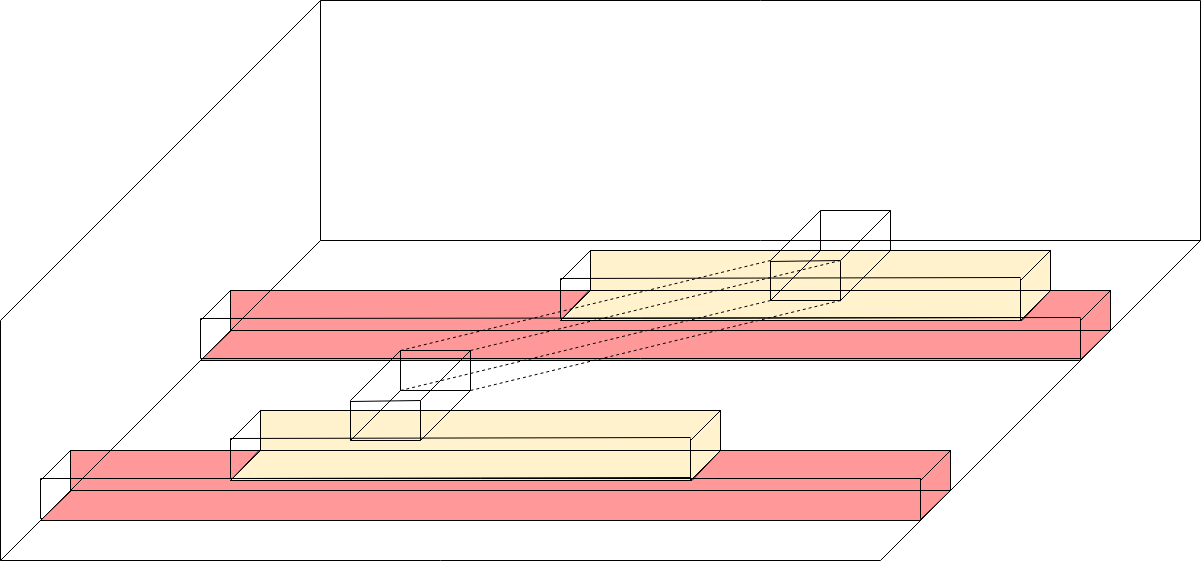
\includegraphics[scale=0.3]{img/Problembeschreibung/flamegraph_3D.png}
	\caption[3D Flammengraph]{Skizzierung eines dreidimensionalen Flammengraphs mit Nachrichtenaustausch}
	\label{fig:flamegraph_3D}
\end{figure}

\begin{figure}[!ht]
	\centering
	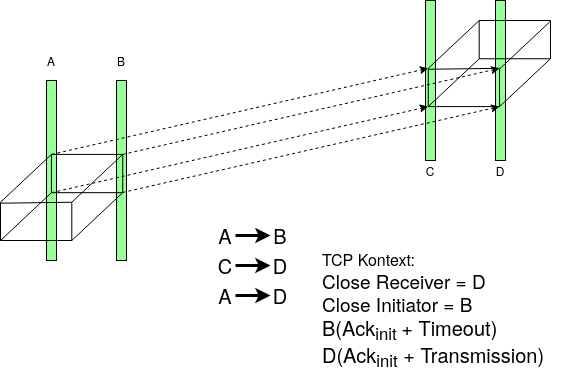
\includegraphics[scale=0.5]{img/Problembeschreibung/flamegraph_3D_closing.png}
	\caption[Flammengraph TCP schließung]{Detailierte Betrachtung des in \cref{fig:flamegraph_3D} gezeigte Nachrichtenaustauschs. Stellt die Schließung einer TCP Verbindung dar}
	\label{fig:flamegraph_3D_closing}
\end{figure}

\section{Kontextproblem von Events}
\label{section: Kontextproblem von Events}

\section{Anforderungsanalyse}
\label{section:Anforderungsanalyse}

Das Systems, für das die Instrumentalisierungsbilbiothek entwickelt wird, ist ein System für verteiltes Rendering. Die Instrumentalisierungsbilbiothek muss notwendige Funktionalitäten spezifizieren, die es ermöglichen ein Modell aus kausal abhängigen Events darzustellen. Zur Erstellung des Modells muss sich mit den Funktionalitäten der \textbf{Eventgenerierung}, der \textbf{Eventrelation}, der \textbf{Synchronisation von Eventgeneratoren}, der \textbf{Eventübermittlnug} und der \textbf{Ordnung von Events} beschäftigt werden. Im Fokus der Interpretation des Modells soll die \textbf{end-zu-end Latenz}, sowie die \textbf{Generierungszeit eines Frames} stehen. Rahmenbedingungen wie die eingeschränkte \textbf{Nachrichtenmodifikation} sind zu berücksichtigen.

Semantisch relevante Ereignisse sind zu definieren. Eine Funktionalität muss geschaffen werden, die es erlaubt, diese Ereginisse als ein Event abzubilden. Die Generierungfunktionalität muss dafür sorgen, dass die Events einem spezifizierten Aufbau aufweisen, um weiterverarbeitet und ausgewertet werden zu können. Die Nutzung einer standarisierten und erprobten \gls{apiLabel} ist wünschenswert.
 
\subsection{Funktionalitäten}

\subsubsection{Eventgenerierung}
\label{section:Eventgenerierung}
Events müssen in einem für die Anwendung semantisch relevanten Bereich generiert werden können. 

\subsubsection{Eventrelation}
\label{subsection:Eventkorrelation}
Es muss ein Modell für Events konzipiert werden. Das Modell muss in der Lage sein, Relationen abbilden zu können. Diese Relationen sollen die kausalen Zusammenhänge der Events darstellen. 

\subsubsection{Synchronistion von Eventgeneratoren}
\label{subsection:Synchronistion von Eventgeneratoren}
Eventgeneratoren sind oftmals auf verschiedenen Komponenten des verteilten Systems angesiedelt. Wie kann also ein Konzept aussehen, dass dafür sorgt, dass Events geordnet werden können.

\subsubsection{Eventübermittlung}
\label{section:Eventübermittlung}
Damit ein Kausalpfad erstellt werden kann, müssen die verstreuten Events in einer Form zusammengeführt werden können.

\subsubsection{Eventordnung}

\subsection{Interpretation des Modells}

\subsubsection{end-zu-end Latenz}

\subsubsection{Generierungszeit eines Frames}
Die Renderinggeschwindigkeit wird anhand der Zeit gemessen, also wieviele \emph{ms} gebraucht werden, um ein Bild zu generieren. gemessen Der Generierungsprozess eines \emph{Frames} umfasst vier Ebenen. Diese Ebenen sind die Applikationsebene, die Geometrieprozessierung, die Rasterung und die Pixelprozessierung. Die Verarbeitung wird, abhängig von der bearbeitet Ebene, von der \gls{cpuLabel} oder der \gls{gpuLabel} durchgeführt. Es ist wünschenswert GPU und CPU Aktivitäten überwachen zu können.

\subsubsection{Nachrichtenmodifikation}

Die Generierung von Events kann von zwei Perspektiven aus betrachtet werden.
Zum einen die \emph{Blackbox} Perspektive und zum anderen die \emph{Whitebox} Perspektive.

Bei dem Blackboxansatz, wird die Generierung angestoßen, sobald Schnittstellen angesprochen werden. Dabei werden betriebssystemspezifische Funktionalitäten genutzt, um diese Betriebssystemereignisse zu erkennen. Diese Ereginisse können erkannt, aufgearbeitet und als Events gespeichert werden. Betriebssystemspezifische Ereignisse sind vorallem ausgehende und eingehende Nachrichten, die von den Netzwerkschnittstellen verarbeitet werden. \cref{fig:distributed_system_network} zeigt eine auf dem TCP/IP Stack basierende Nachricht. Die Daten der Senderadresse, der Empfängeradresse und einem Zeitstempel könnten genutzt werden. Allerdings ist das Fehlen von Applikationsinformationen ein entscheidendes Problem. Das Ziel des Blackboxansatz ist die minimale Vorraussetzung von \emph{a priori} Informationenen über Kommunikationswege, über den Aufbau von Applikationsnachrichten, die Semantik der Anwendung und den Aufbau des verteilten Systems.\footpartcite{Aguilera2003}. Allerdings sind diese Daten äußert wichtig, um ein tiefgreifendes Verstädnis des verteilten Systems zu gewinnen. 

Der Whiteboxansatz nutzt Instrumentalisierung des Quellcodes, um die Eventgeneriernug anzustoßen. Dabei wird vorausgesetzt, dass die Semantik der Anwendung, Informationen über den Aufbau von Nachrichten, den Aufbau des Systems und die Kommunikationswege zwischen Komponenten bekannt sind. Bei der Notwendigkeit einer Modifizierung von Nachrichten weist dieser Ansatz jedoch auch schwächen auf. Im Anwendungsfall des verteilten rendering Systems fehlt die Möglichkeit, Nachrichten, innerhalb der Anwendung, um Tracingdaten zu erweitern.


% ----------------------------------------------------------------------------

% ----------------------------------------------------------------------------
% Copyright (c) 2016 by Burkhardt Renz. All rights reserved.
% Die Vorlage für eine Abschlussarbeit in der Informatik am Fachbereich
% MNI der THM ist lizenziert unter einer Creative Commons
% Namensnennung-Nicht kommerziell 4.0 International Lizenz.
%
% Id:$
% ----------------------------------------------------------------------------

\chapter{Design}
\label{chapter:Design}
In diesem Kapitel werden die in \cref{chapter:Problembeschreibung} beschriebenen Problemstellung bearbeitet. Anfänglich werden Designziele definiert, die den Rahmen für die Konzipierung bilden. In \cref{section:Datenmodell} wird ein Datenmodell vorgestellt, welches sich an Standards von bereits existierenden Tracingmodellen orientiert. \cref{section:Verarbeitungsmodell} präsentiert ein Konzept zur Verarbeitung der erhobenen Tracingdaten. Der \cref{section:Visualisierung} beschäftigt sich mit der Darstellung der Tracingdaten zur Informationsgewinnung durch den Anwender der Bibliothek. Somit wird ein Konzept für die Tracinginfrastruktur \textbf{Traktor }zur Erhebung, Verarbeitung und Visualisierung von Tracingdaten vorgestellt.

\section{Designziele}
\label{section:Designziele}

Aus den in \cref{section:Anforderungsanalyse} beschriebenen Anforderungen folgen Designziele, die an die Implementierung gestellt werden. Die von Google erstellte Fachpublikation \emph{Dapper, a Large-Scale Distributed Systems Tracing Infrastructure}\footpartcite{Shanbhag2010} dient vielen Tracingsystemen als konzeptionelle Grundlage. In der Puplikation werden Designziele aufgeführt, die neue Tracingsysteme bewerten sollten. Aus den Anforderungen des verteilten Rendering-Systems ergeben sich Designziele. Diese Designziele umfassen die (\lowroman{1}) \textbf{Verarbeitungskosten}, die (\lowroman{2}) \textbf{Benutzbarkeit}, die (\lowroman{3}) \textbf{Portabilität} und die (\lowroman{4}) \textbf{Datenverfügbarkeit}. Ausserdem werden Nicht-Ziele definiert. Zu diesen gehören die (\lowroman{5}) \textbf{Anwendungs-Level Transparenz} und die (\lowroman{6}) \textbf{Skalierbarkeit}.

\subsection{Ziele}
\label{subsection:Ziele}
\textbf{Verarbeitungskosten} \space\space\space Ein für die Performance der Anwendung kritisches Designziel, in der Tracing eingeführt werden soll, stellt der \textbf{Overhead} dar. Der Overhead, der durch die Instrumentalisierung entsteht, soll möglichst gering sein. So kann etwa in spezialisierten hochperfomanten Services kleinster, durch Instrumentalisierung entstehender Mehraufwand, deutlich merkbar sein.\footpartcite{Shanbhag2010}. 

\textbf{Benutzbarkeit} \space\space\space Die Benutzbarkeit des Tracingsystems soll durch die Verwendung von Standards gewährleistet sein. Die von \emph{Opentracing} veröffentlichte \gls{apiLabel} soll der Instrumentalisierungsbibliothek eine vertraute und bewährte Anwendererfahrung liefern. 

\textbf{Portabilität} \space\space\space Ein weiteres Designziel soll eine gegebene \textbf{Portabilität} sein. Die Umgebung für die das Tracingsystem entwickelt wird, ist eine Mischung aus plattformabhängigen und plattformunabhängigen Komponenten. Durch den verminderten Mehraufwand der bei plattformunabhängigen Komponenten entsteht, wird eine verbesserte Nutzerfreundlichkeit gewährleistet. Vor allem bei der Integration in bestehende Systeme wird dies bemerkbar, da Bauprozesse von Projekten plattformabhängig sind. Der platformabhängige Bauprozess soll im Falle des verteilten rendering System nicht beeinflusst werden. 

\textbf{Datenverfügbarkeit} \space\space\space Die Datenverfügbarkeit soll zeitnah stattfinden. Die von der Tracinginfrastruktur generierten Tracingdaten sollen zur Laufzeit dargestellt werden. 

\subsection{Nicht-Ziele}
\label{subsection:Nicht-Ziele}

Die von Dapper genannten Designziele der \emph{Anwendungs-Level Transparenz} und der \emph{Skalierbarkeit} spielen für das verteilte Rendering-System eine untergeordnete Rolle. Diese Bewertung hat ihren Ursprung aus einer interpretierten Form eines Sprichworts. 

\begin{quote}
	\cbstart
	Du bist nicht Google, also versuch auch nicht Google zu sein
	\cbend
\end{quote}

Dapper ist für eine Infrastruktur konzipiert, die globalen  Maßstäben entspricht. Das verteilte rendering System entspricht nicht diesen Maßstäben, somit soll auch die Tracinginfrastruktur diese nicht erfüllen müssen. Die beiden Deisgnziele von Dapper werden als Nicht-Ziele für das verteilte rendering System bewertet.

\textbf{Anwendungs-Level Transparenz}\space\space\space Instrumentalisierung erfordert Eingreifen in Anwendungsquellcode. Dapper löst dies durch Nutzung von Bibliotheken. Diese werden instrumentalisiert und in der Anwendungslogik verwendet. Somit ist die Tracinginfrastruktur für den Anwendungsentwickler nicht wahrnehmbar. Die Instrumentalisierung des verteilten Rendering-Systems soll an semantisch relevanten Bereichen stattfinden und flexibel sein. Dies gelingt durch direktes Modifizieren der Anwendungslogik. Der Anwendungsentwickler muss sich dementsprechend selbst um die Instrumentalisierung kümmern. 

\textbf{Skalierbarkeit} \space\space\space Der Aufbau des verteilte rendering System ist, in seiner einfachsten Form, statisch. Das bedeutet, dass eine Skalierbarkeit keine zentrale Rolle in dem Design der Tracinginfrastruktur darstellt. Die Skalierbarkeit soll allerdings bewertet werden. 

\section{Datenmodell}
\label{section:Datenmodell}

In diesem Abschnitt wird der Lösungsansatz der Frage \textbf{F1} diskutiert.
Diese Frage erfordert die Konzipierung eines Datenmodells, welches drei Aspekte berücksichtigt. Der erste Aspekt wird durch die Zeitspanne des Events selbst dargestellt. Dabei muss das Event derart repräsentiert werden, sodass eine Zeitspanne als Information daraus gewonnen werden kann. Die detaillierte Darstellung wird in \cref{subsection:Spans} erläutert. Der zweite Aspekt entsteht durch die Gegebenheit eines lokalen Kontexts. Dieser wird in \cref{subsection:Tracingcontext innerhalb eines Systems} beschrieben. Der dritte Aspekt ist durch die Kommunikation von Komponenten des Systems gegeben. Dieser wird  in \cref{subsection:Tracingcontext über Systemgrenzen} dargestellt.


Das Datenmodell beruht auf dem Spanmodell, welches in der vorher beschrieben Fachpublikation \emph{Dapper} vorgestellt, durch die Spezifikation von \emph{Opentracing} erweitert und dem Anwendungsfall des verteilten Rendering-Systems und des Entwicklungsprojekts angepasst wird.

Ein Überblick über das Spanmodell wird gezeigt. Ein \emph{Trace} bildet die größte Einheit des Modells ab. Traces sind Eventsammlungen, die den Weg einer Anfrage durch ein verteiltes System darstellen. Ein Trace ist die Reise der Anfrage, wohingegen einzelne Events die Etappen dieser Reise sind. Die Events werden weiterführend als Spans bezeichnet.  Ein Trace beinhaltet ein bis beliebig viele \emph{Spans}. Ein Span ist die kleinste Einheit eines Traces. Spans bilden einen Arbeitsprozess innerhalb eines Prozesses ab. Innerhalb eines \emph{Threads} ist zu jeder Zeit nur ein Span \emph{aktiv}.


\subsection{Spans}
\label{subsection:Spans}
Um Daten zu repräsentieren und zusammenzufassen, braucht es einen Datencontainer. Die Datencontainer eines Traces sind Spans. Spans beinhalten die Daten die nötig sind, um eine Reihenfolge herzustellen. Außerdem besteht die Möglichkeit Anwendungsinformationen, wie zum Beispiel Anwendungslogs, in Spans mitzuführen.

Ein Span kapselt folgende Informationen:
\begin{itemize}
	\item Ein Operationsnamen
	\item Ein Startzeitpunkt
	\item Ein Endzeitpunkt
	\item Ein Spankontext
\end{itemize}

\begin{figure}
	\centering
	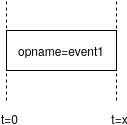
\includegraphics[scale=0.7]{img/Design/Span.png}
	\caption[Zeitliche Darstellung eines Spans]{Darstellung eines Spans mit Anfangszeit, Endzeit und Operationsnamen}
	\label{fig:Span}
\end{figure}

Der Spankontext wiederum ist auch ein Datencontainer. Dieser beinhaltet eine \emph{SpanID} und eine \emph{TraceID}. Auch ein Beziehungstyp wird mitgeführt. Der Beziehungstyp kann zum einen eine \emph{Child-of} Beziehung oder eine \emph{Follows-From} Beziehung annehmen. Diese beiden Beziehungstypen ergeben sich aus der zeitlich Anordnung von Events. Die in \cref{subsection:Ordnung von Events} beschriebene Ordnung  bieten die Grundlage für die Unterscheidung dieser beiden Beziehungstypen. $t1$ ist der Beginn von Span A. Innerhalb dieses Events findet ein weiteres Event statt. Dieses wird durch Span B repräsentiert und ist zeitlich durch $t2$ und $t3$ markiert. Anschließend beendet Span A zum Zeitpunkt $t4$. Span B ist ein Kindspan von Span A, weil sie von Span A ausgelöst worden ist und noch vor Span A beendet. Eine Follows-From Beziehung äußert sich dahingehend, dass ein Span auf einen anderen folgt und eine Kausalität gegeben ist. Span C startet zum Zeitpunkt $t5$ und endet zum Zeitpunkt $t6$. Durch die Anwendungslogik, die Span C umfasst, wird Span D generiert, nachdem Span C beendet wurde. Span D erbt den Kontext von Span C. Die Zeitspanne von Span D ist durch $t7$ und $t8$ dargestellt.
 
\begin{figure}[]
	\centering
	\begin{subfigure}[t]{.49\linewidth}
		\centering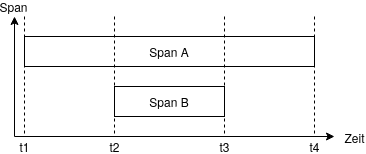
\includegraphics[width=.8\linewidth]{img/Design/SpanBeziehungstypenA.png}
		\caption[Abbildung]{Span B hält eine \emph{Child-Of} Beziehung zu dem Elternspan}
		\label{fig:SpanBeziehungstypenA}
	\end{subfigure}
	\begin{subfigure}[t]{.49\linewidth}
		\centering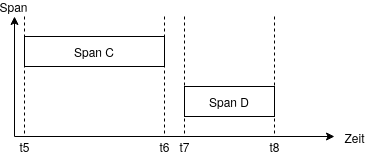
\includegraphics[width=.8\linewidth]{img/Design/SpanBeziehungstypenB.png}
		\caption[Abbildung]{Span D hält eine \emph{Follows-From} Beziehung zu Span C}
		\label{fig:SpanBeziehungstypenB}
	\end{subfigure}
	\caption[Darstellung der zeitlichen Anordnung der Beziehungstypen \emph{Child-Of} und  \emph{Follows-From}]{}
\end{figure} 


Die SpanId ist eine eindeutig identifizierbare Nummer, die bei der Erstellung eines Spans generiert und in dem Spankontext gespeichert wird. Die TraceId ist eine eindeutig identifizierbare Nummer, die bei der Erstellung des ersten Spans eines Traces erstellt wird. Die TraceId wird auch in dem Spankontext gespeichert. Nachfolgende Spans, die zu diesem Trace gehören, übernehmen die TraceId. Dadurch ist eine Zuordnung jedes Spans zu einem Trace gegeben. Die zeitliche Einordnung des Startzeitpunktes und des Endzeitpunktes eines Spans ist in  \cref{fig:Span} dargestellt. Die Konzipierung der Start- und Endzeit sind die zentralen Daten, mit der sich Fragestellung \textbf{F1} lösen lässt. Durch die Relationbildung mittels einer Beziehungstypdefinition und der Zeitstempel, ist eine Zeitmessung von Eventzeitspannen gegeben. Das Beispiel aus \cref{fig:Eventzeitspannen} verdeutlicht dies. Die Gesamtzeit eines Events bzw. eines Spans lässt sich durch die Differenz zweier Zeitstempel ermitteln. Die Zeitspanne die von dem Span \emph{FormatiereNachricht} eingenommen wird, ergibt sich aus $t3 - t2$. Dies wäre ein Event mit einer Lebensdauer von 0.5. Die Relationstypen werden dazu genutzt, um den Zustand des Traces zu definieren. Ein Trace ist dann abgeschlossen, sobald der letzte Span eines Traces, ohne \emph{Child-Of} Beziehung beendet ist. \emph{EmpfangeAntwort} ist in diesem Fall der letzte Span. Außerdem besitzt dieser keinen übergeordneten Span, gegeben aus einer \emph{Follows-From} Beziehung zum Ursprungsspan. Daraus folgert der Abschluss des Traces.

\begin{figure}[!b]
	\centering
	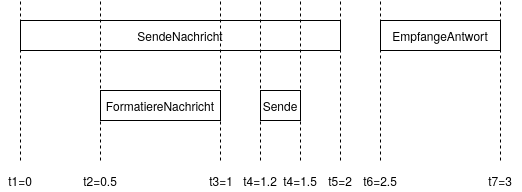
\includegraphics[scale=0.7]{img/Design/Eventzeitspannen.png}
	\caption[Zeitmessung von Spans eines Traces]{Darstellung eines Trace mit mehreren Spans. Anfangszeit und Endzeit ergeben die Gesamtzeit eines Traces}
	\label{fig:Eventzeitspannen}
\end{figure}



\subsection{Tracingcontext innerhalb eines Systems}
\label{subsection:Tracingcontext innerhalb eines Systems}

\begin{figure}[!ht]
	\centering
	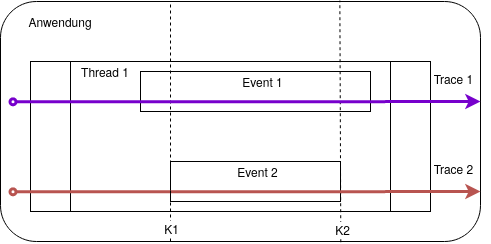
\includegraphics[scale=0.5]{img/Design/SpanThreadKontext.png}
	\caption[Tracingkontexts in einem Threads innerhalb einer Anwendung]{Anwendung mit einem Thread. Ein von der Instrumentalisierung veranlasster Kontextwechsel innerhalb eines Threads}
	\label{fig:SpanThreadKontext}
\end{figure}


Ein Prozess kann \emph{Threads} implementieren. Die Events, die in einem Thread stattfinden, können ihren Lebenszyklus entweder in diesem beginnen und beenden oder in einem Thread beginnen und in einem anderen Thread enden. Der Tracer, also die übergeordnete Verwaltungseinheit, muss jedoch jederzeit feststellen können, welches Event \emph{aktiv} ist. Der Grund dafür ist beispielsweise das Erstellen von Relationen für zu generierende Events, die ihr Elternevent kennen müssen. Eine Umgebung ist notwendig, in der der aktive Span festgestellt werden kann. Diese Umgebung wird als \emph{Scope} bezeichnet. Der Kontext eines Traces ergibt sich aus dem aktiven Span. Der Kontext ist notwendig, um folgende Spans zuordnen zu können. Anhand der aufgeführten Beispiele wird das Konzept des Scopes verdeutlicht. Dabei beinhaltet das erste Beispiel, dargestellt in \cref{fig:SpanThreadKontext}, einen Thread, indem zwei Traces parallel existieren. Die \cref{fig:SpanMultipleThreadKontext} stellt die Situation eines Traces über mehrere Threads dar.

Im ersten Beisiel sei gegeben, dass eine Anwendung ein Thread implementiert. Dabei existieren zwei parallele Traces. Trace 1 beinhaltet das Event 1. Event 1 sendet asynchron eine große Datei an ein Frontend, wie dies in dem verteilten Rendering-System der Fall sein könnte.  Trace 2 beinhaltet Event 2. Event 2 liest eine kleinen Datei aus einem Speicher. Es wird davon ausgegangen, dass das Schreiben deutlich mehr Zeit beansprucht, als das Lesen. Der Ablauf des Kontextwechsels beginnt mit der Erstellung und Aktivierung des Spans, welcher Event 1 umfasst. Die Aktivierung des Spans sorgt dafür, dass dieser in den \emph{Scope} wandert. Der Scope verwaltet den aktiven Span. Die Startzeit des Spans wird gespeichert und die Anwendungslogik asynchron bearbeitet. Event 2, welches zu Trace 2 gehört, startet und generiert den zweiten Span. Dabei findet der Kontextwechsel K1 statt. K1 tauscht den Span von Event 1 mit dem Span von Event 2. Der Span von Event 2 ist nun aktiv und der Span von Event 1 nimmt implizit den Zustand \emph{nicht beendet} ein. Die Anwendungslogik, die Event 2 darstellt, wird bearbeitet. Das Event 2 beendet, woraus die Schließung des dazugehörigen Spans folgert. Die Endzeit wird gespeichert. Trace 2 schließt, da der Span von Event 2 keinen \emph{ElternId} beinhaltet und somit der Wurzelspan ist. K2 wechselt wieder den aktiven Span. Danach beendet Event 1, da der \emph{Callback}, durch die Beendigung des Schreibens, aufgerufen wird. Entsprechenden schließt Span von Event 1. Auch hier ist dieser der Elternspan und schließt Trace 1 ab. Zu jedem Zeitpunkt kann des Tracerobjekt feststelle, welches das aktive Span ist.


\begin{figure}[!ht]
	\centering
	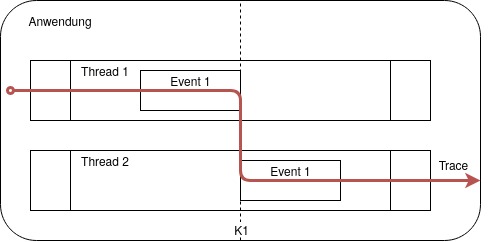
\includegraphics[scale=0.5]{img/Design/SpanMultipleThreadKontext.png}
	\caption[Tracingkontexts über mehrere Threads innerhalb einer Anwendung]{Anwendung mit zwei Threads. Ein von der Instrumentalisierung veranlasster Kontextwechsel zwischen Threads}
	\label{fig:SpanMultipleThreadKontext}
\end{figure}

Im zweiten Beispiel sei gegeben, dass eine Anwendung zwei Threads implementiert. Es exisitert ein Trace, welches Event 1 beinhaltet. Thread 1 beinhaltet Event 1. Event 1 sorgt für die die Erstellung eines Scopes in dem der Span von Event 1 erstellt und aktiviert wird. Kontextwechsel K1 findet statt. Der Scope in Thread 1 schließt. Da Event 1 in Thread 2 weitergeführt wird, beendet der Span nicht bei K1. In Thread 2 findet die Weiterführung von Event 1 statt, weshalb ein Scope eröffnet wird. In diesem Scope wird der in dem vorherigen Scope aktive Span eingeführt. Dies stellt die Kontextübermittlung dar. Event 1 endet anschließend und Trace 1 wird geschlossen.

Diese beiden Beispiele zeigen die Relevanz von Scopes zur Verfolgung des Kontexts innerhalb eines Systems ohne Netzwerkkommunikation. Scopes lösen das Problem der lokalen  Kontextverfolgbarkeit. Damit lassen sich Endzeiten von Spans innerhalb eines Systems, auch über Threadgrenzen hinaus, bestimmen. 

\subsection{Tracingcontext über Prozessgrenzen}
\label{subsection:Tracingcontext über Systemgrenzen}

Die Kontextverfolgung über Prozessgrenzen stellt wohl das schwierigste Problem im verteilten tracing dar. Im Fokus steht hierbei die Fragestellung \textbf{F3}. Es werden zwei Konzepte vorgestellt, die es ermöglichen sollen, den Tracingkontext über Prozessgrenzen hinaus zu transportieren. 


\subsubsection{Registry}
Das erste Konzept ist die \textbf{Traktor Registry}. 
Der Infrastrukturaufbau, bestehend aus der Registry und den Tracern, die mit der Registry verbunden sind, erfüllt die Aufgabe der Kontextpropagierung. Die Traktor Registry dient als Nachrichtenproxy für die Tracer-Instanzen. Bei der Initialisierung einer Traktorinstanz stellt diese eine Websocketverbindung zur Registry her. Bei eingeleiteter Kontextpropagierung wird eine Websocketnachricht, die den Tracekontext beinhaltet, an die Registry gesendet. Die Registry empfängt die Nachricht und sendet diese an ihr Zieltracer weiter. Der Zieltracer, der auch eine Verbindung zur Registry aufgebaut hat, empfängt die Nachricht. Der Nachrichteninhalt wird extrahiert und für die Erstellung für kommende Spans des aktuellen Traces und der damit verbundenen Relationsbildung genutzt. Die Verarbeitungsablauf dieses Registryservices lässt sich aus \cref{fig:Traktor-Registry} erschließen.

\begin{figure}[!ht]
	\centering
	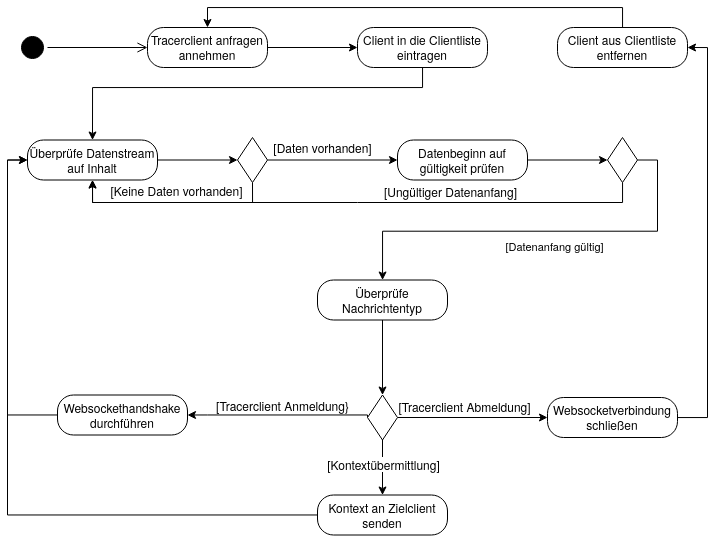
\includegraphics[scale=0.65]{img/Design/Traktor-Registry.png}
	\caption[Aktivitätendiagramm der Traktor Registry]{Aktivitätendiagramm der Traktor Registry}
	\label{fig:Traktor-Registry}
\end{figure}

\subsubsection{Interceptor}
Das zweite Konzept beruht auf dem Abfangen und dem Modifizieren von spezifizierten Nachrichten, die aus dem System gesendet werden. Es werden betriebssystemabähngige Funktionalitäten genutzt, um ausgehende Nachrichten zu identifizieren und einzuordnen. Dabei wird auf Nachrichten gelauscht, die von einem Port ausgehen, die die Anwendungskomponente belegt. Entspricht diese Nachricht den Vorgaben, kann diese um Kontextdaten erweitert werden. Anschließend wird die Nachricht in modifizierter Form an ihren Empfänger weitergeleitet. Auf dem Empfängersystem sitzt ein gleicher \emph{Interceptor}. Dieser lauscht auf auf eingehende Nachrichten und filtert, wie beim Senden, die gewünschten Nachrichten heraus. Der Tracingkontext wird aus der Nachricht extrahiert. Anschließend wird die Nachricht, so wie sie von der Senderanwendung geschickt wurde, an die Empfängeranwendung weitergeleitet. \cref{fig:Nachrichteninterceptor} zeigt die Nachrichtenmodifikation, bei der eine Anwendung auf dem Sendersystem Nachrichten über die Ports 8080 und 8090 an eine Empfängeranwendung sendet. Ports die nicht von der Anwendung beansprucht werden, wie zum Beispiel Port 1337, sind von der Modifikation nicht betroffen. Der Interceptor erweitert die Nachrichten um den Trancingkontext, welches von dem Emfpängerinterceptor entpackt werden. Durch diese Funktionalität lässt sich die Registry als potentielle zentrale Fehlerquelle ersetzten. Allerdings werden dazu auf jedem System zusätzliche, neben der Anwendung laufende, Scripte benötigt.

 \begin{figure}[]
 	\centering
 	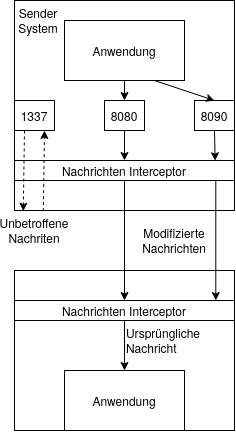
\includegraphics[scale=0.6]{img/Design/Nachrichteninterceptor.png}
 	\caption[Design des Nachrichteninterceptor]{Design des Nachrichteninterceptor}
 	\label{fig:Nachrichteninterceptor}
 \end{figure}

\section{Verarbeitungsmodell}
\label{section:Verarbeitungsmodell}
Das Verarbeitungsmodell ist das Bindeglied zwischen Visualisierung und Instrumentalisierung. Dabei sind zwei Komponenten zu designen. Die erste Komponente hat dafür zu sorgen, dass die Daten aus der Anwendung gelangen und zu einem Service übermittelt werden, der die Daten sammelt. Dafür werden \emph{Reporter} eingesetzt. Die zweite Komponente ist der \emph{Kollektor}. Dieser erhält alle Daten der Reporter. Die gesammelten Daten werden in eine strukturierte Form aufgearbeitet. Anschließend können die Daten, abhängig von der Konfiguration, gespeichert oder direkt visualisiert werden.

\subsection{Reporter}
\label{subsection:Reporter}
Bei Abschluss eines Spans wird dieser an den Reporter übermittelt. Durch eine UDP Verbindung zu dem Kollektor werden die Spans versendet. Der Trace wird von der Verwaltungseinheit parallel weitergeführt, bis dieser abgeschlossen ist. Der Reporter kennt den Zustand des gesamten Traces nicht. 

\subsection{Kollektor}
\label{subsection:Kollektor}
Der Kollektor ist ein eigener Service im verteilten System. In dem Kollektor werden die reporteten Spans gesammelt. Der Kollektor stellt einen UDP Endpunkt bereit, über den die Reporter daten übermitteln können. Diese können in einer relationalen Datenbank gespeichert werden. Das Datenmodell der Traces und Spans bietet sich dafür an. Anhand der TraceId lassen sich die dazugehörigen Spans ermitteln. Jede TraceId ist ein Eintrag in der Datenbank. Die Datenverfügbarkeit ist entsprechend gegeben.  

\section{Visualisierung}
\label{section:Visualisierung}
In diesem Kapitel sollen Darstellungsformen von Tracingdaten präsentiert werden. Dabei werden bestehende Visualisierungsmöglichkeiten von Performancedaten aufgegriffen und dem Kontext von distributed tracing, sowie dem verteilten Rendering-System angepasst.


\subsection{Frame Galerie}

Das verteilte Rendering-System generiert Frames. Die Instrumentalisierung des System hat den Zweck einzelne Frames untersuchen zu können. Eine abstrakte Darstellung der Tracingdaten zur Untersuchung der Frames bietet sich daher an. Bereits existierende Tracingdarstellungen, bietet eine sehr eingeschränkte und spezifizierte Ansicht der Daten. Das Konzept der Frame Galerie soll die Daten interpretieren und für den Anwender eine Abstraktion der Tracingdaten bereitstellen. 

Das Visualisierungskonzept ist durch drei Ebenen gekennzeichnet. Jede Ebene liefert einen gewissen Grad von Informationen. Dabei bietet die oberste Ebene, dargestellt in \cref{fig:FrameGalerieObereEbene}, eine Übersicht über alle Frames. Grenzwertüberschreitungen könne beispielsweise ein Indiz für fehlerhafte Frames sein, die es weiter zu untersuchen gilt. Da nur ein 

\begin{figure}[!ht]
	\centering
	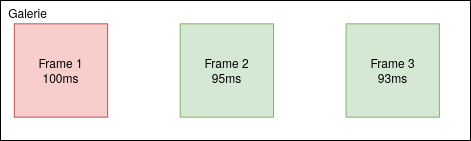
\includegraphics[scale=0.8]{img/Design/FrameGalerieObereEbene.png}
	\caption[Oberste Ebene der Frame Galerie]{ Skizzierung der oberste Ebene der Frame Galerie}
	\label{fig:FrameGalerieObereEbene}
\end{figure}

Da das verteilte Rendering-System konzeptionell in der Lage sein soll, Frames aus Teilframes zusammenzustellen, ist es sinnvoll, den Generierungsprozess der fertigestellten Frames nachvollziehen zu können. Dieser Visualisierungsansatz ist nur dann sinnvoll, sobald die Architektur mehrere Renderer und Aggregatoren umfasst. Aggregatoren wären Systemkomponenten, die die Teilframes sammelt und zusammenführt. Die mittlere Ebene, dargestellt in \cref{fig:FrameGalerieMittlereEbene},  veranschaulicht den Ursprung durch ein Stammbaum. Es müssen nicht alle Teilframes, aufgrund ihres zeitlichen Auftretens in der Generierungsphase, bei der Zusammenstellung verwendet werden. Zusätzlich sind die Generierungszeiten aus den Tracingdaten hergeleitet und an die jeweiligen Frames geheftet. Bei einem Grenzwertübertritt werden diese farblich hervorgehoben.

\begin{figure}[!ht]
	\centering
	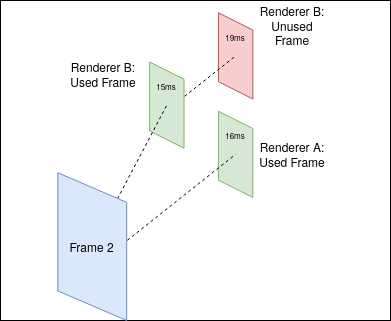
\includegraphics[scale=0.8]{img/Design/FrameGalerieMittlereEbene.png}
	\caption[Mittlere Ebene der Frame Galerie]{ Skizzierung der mittleren Ebene der Frame Galerie}
	\label{fig:FrameGalerieMittlereEbene}
\end{figure}

Die unterste Ebene ist Detailansicht der Spans. Hierzu wird die klassische Visualisierungform von Tracingdaten verwendet. Die Servicenamen, die Operationsnamen und die dazugehörigen Verarbeitungszeiten der Spans sind erkenntlich. Zusätzlich können \emph{Breakpoints} gekennzeichnet werden. Durch Visualisierung von beispielsweise gestrichelten Linien, wie in \cref{fig:FrameGalerieUntereEbene1} gezeigt, ist ersichtlich, dass Frames, die ab diesem Zeitpunkt generiert werden, für die Zusammenführung ungenutzt bleiben.

Dem Anwender der Visualisierung ist durch die Ebenenaufteilung möglich, für ihn interessante Aspekte auszuwählen und gegebenenfalls Fehlerquellen weitergehend zu untersuchen.

\begin{figure}[!ht]
	\centering
	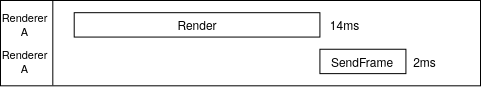
\includegraphics[scale=0.8]{img/Design/FrameGalerieUntereEbene2.png}
	\caption[Untere Ebene der Frame Galerie: Beispiel 2]{ Skizzierung der unteren Ebene von Teilframe aus Renderer A}
	\label{fig:FrameGalerieUntereEbene1}
\end{figure}
\begin{figure}[!ht]
	\centering
	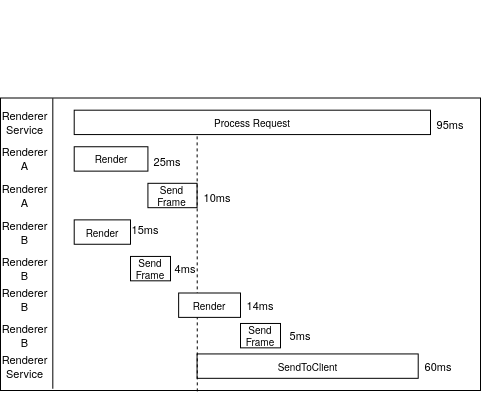
\includegraphics[scale=0.8]{img/Design/FrameGalerieUntereEbene1.png}
	\caption[Untere Ebene der Frame Galerie: Beispiel 1]{ Skizzierung der unteren Ebene von Frame 2}
	\label{fig:FrameGalerieUntereEbene2}
\end{figure}

\subsection{Dreidimensionaler Flammengraph}
\label{subsection:Dreidimensionale Flammengraphen}

Das zweite Visualisierungskonzept nimmt sich Flammengraphen, gezeigt in \cref{fig:flamegraph_3D}, und Sequenzdiagramme als Vorbild.

Dabei werden Spans aufeinandergestapelt. Spans werden als rechteckige Flächen dargestellt und farblich hervorgehoben.	Diese werden anhand ihrer Berarbeitungsreihenfolge geordnet. Je tiefer die Operation in dem Tracestack ist, desto höher ist diese im Graph. Diese Eigenschaft wird mit dem klassichen Flammengraph geteilt. Spans werden zudem durch Services, in denen sie generiert wurden, aufgeteilt. Die Relationen zueinander, sind durch Linien gekennzeichnet. Dadurch lassen sich Kausalitäten zwischen Spans, sowie die dazugehörigen Services feststellen.

\begin{figure}[!ht]
	\centering
	\hspace*{-2cm}  
	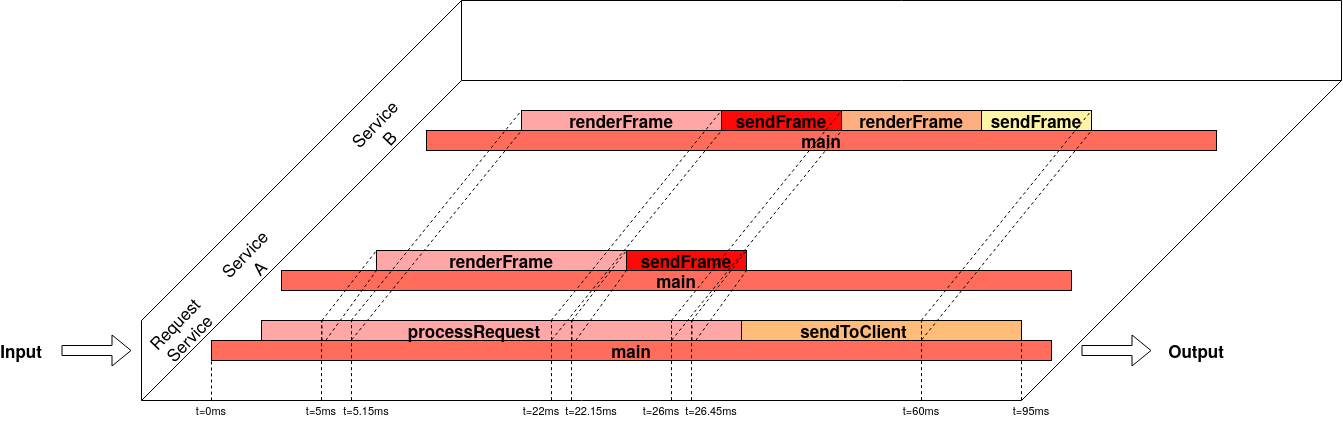
\includegraphics[scale=0.36]{img/Design/3D-Flammengraph-Konzept.png}
	\caption[Darstellungsbeispiel eines 3D-Flammengraph ]{ Darstellungsbeispiel eines 3D-Flammengraph}
	\label{fig:3D-Flammengraph-Konzept}
\end{figure}

Diese Visualisierungsform soll ein Vergleich zwischen Traces ermöglichen. Die Traces werden zusammen auf eine Zeitachse gestellt. Der Anweder kann die Traces anschließend vergleichen. Dadurch sollen nicht verwendete Frames identifizerbar sein. Auch die Ursache soll damit ermittelt werden können. Spezielle Zustände des verteilten verteilten rendering System, wie zum Beispiel dem Setzen einer neuen Kameraposition, ausgelöst durch den Client, können näher untersucht werden. Das Setzen ist eine asynchrone Funktionalität, die im rendering System dazu führt, dass eine neue Framegenerierung angestoßen wird. Dabei werden allerdings aktuell bearbeitete Frames nicht gestoppt, sondern fertiggestellt und gesendet. Diese werden nur nicht weiter verwendet. Um die zeitliche Einordnung dieser Events darstellen zu können, müssen die Traces miteinander verglichen werden. In \cref{fig:3D-Flammengraph-Vergleich} wird eine solche Situation gezeigt. Der Trace startet im Requestservice. Der Span mit dem Operationsnamen \emph{processRequest} sorgt im Render Service A für zwei Framegenerierungen. Der erste \emph{generateFrame} Span schließt zum Zeitpunkt \textbf{t1} erfolgreich ab, entsprechend wird der Frame gesendet und verwendet. Die Generierung wird mit dem zweiten generateFrame fortgesetzt. Anschließend wird der erste ProcessRequest durch eine Benutzereingabe zum Zeitpunkt \textbf{t2} unterbrochen. Der zweite Trace beginnt. Der Requestservice veranlasst die Generierung des Frames mit den neuen Benutzerdaten im Render Service B zum Zeitpunkt \textbf{t3}. Der Render Service A stellt seinen Frame zum Zeitpunkt \textbf{t4} fertig. Da der Frame auf Benutzereingaben beruht, die zu diesem Zeitpunkt veraltet sind, wird der Frame nicht weiter verwendet. Trace 1 schließt ab. Währenddessen wird Trace 2 fortgesetzt.

\begin{figure}[!ht]
	\centering
	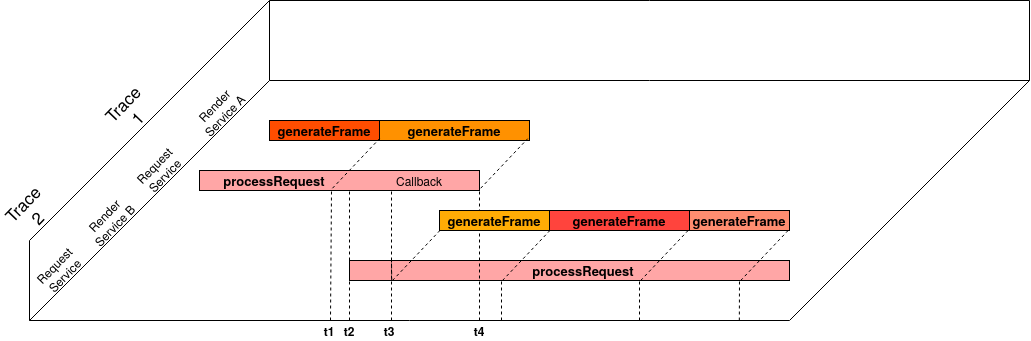
\includegraphics[scale=0.4]{img/Design/3D-Flammengraph-Vergleich.png}
	\caption[Darstellungsbeispiel eines Tracevergleich mit einem 3D Flammengraph]{ Tracevergleich mit einem 3D Flammengraph}
	\label{fig:3D-Flammengraph-Vergleich}
\end{figure}

\section{Trakorentwicklungsumgebung}
\label{section:Trakorentwicklungsumgebung}
In diesem Kapitel wird die Traktorentwicklungsumgebung spezifiziert. Die Umgebung soll die verschiedenen Anwendungsfälle der Traktorbibliothek abdecken. Eine Entwicklungsumgebung ist dahin gehend sinnvoll, dass der Anwendungsfall des verteilten rendering Systems komplexe abhängigkeiten aufweist, bei der eine effiziente Entwicklung, z.B. durch die platformabhängigen Plugins oder der Unityumgebung, beeinträchtigt wird.

Die Traktorentwicklungsumgebung soll folgende Eigenschaften aufweisen:

\begin{itemize}
	\item \textbf{TE}.1 Die Entwicklungsumgebung soll aus mehreren Webservern bestehen
	\item  \textbf{TE}.2 Die Infrastruktur soll auf genau einem Host-System ein verteiltes System abbilden.
	\item  \textbf{TE}.3 Die Webserver-Komponenten der Entwicklungsumgebung soll mit der Traktor-API instrumentalisiert sein.
	\item  \textbf{TE}.4 Das Ansprechen der Entwicklungsumgebung soll durch einen Kommandozeilen HTTP Client ansprechbar und bedienbar sein.
\end{itemize}

Diese Spezifikation ermöglicht das Testen von Funktionalitäten der Traktor Tracingbibliothek. Dabei sollen die (\lowroman{1}) Eventgenerierungfunktionalitäten ausgeführt werden. Ausserdem soll durch durch die Instrumentalisierung von zwei miteinander kommunizierenden Komponenten (\lowroman{2}) die Kontextpropagierung durchgeführt werden. Das umfasst sowohl die lokale Kontextverwaltung, als auch die Kontextpropagierung über Prozessgrenzen hinaus. Zudem sollen die leichtgewichtigen Services, also den Reporter und die Registry, getestet werden. Dabei ist die (\lowroman{3}) Implementierung des Websocketprotokolls innerhalb der Registry, als auch der (\lowroman{4}) Websocketclient des Tracers zu untersuchen. Mit dieser Spezifikation wird ein Untersuchungssystem beschrieben, mit der teilweise die Designziele überprüft werden können. 
% ----------------------------------------------------------------------------

% ----------------------------------------------------------------------------
% Copyright (c) 2016 by Burkhardt Renz. All rights reserved.
% Die Vorlage für eine Abschlussarbeit in der Informatik am Fachbereich
% MNI der THM ist lizenziert unter einer Creative Commons
% Namensnennung-Nicht kommerziell 4.0 International Lizenz.
%
% Id:$
% ----------------------------------------------------------------------------
\chapter{Implementierung}
\label{chapter:Implementierung}

In diesem Kapitel werden Implementierungen von Prototypen gezeigt, die im Kapitel \cref{chapter:Design} besprochen sind. In \cref{section:Instrumentalisierungsbibliothek: Traktor} werden die Implementierungsdetails der Instrumentalisierungsbilbiothek \textbf{Traktor} vorgestellt. In \cref{section:Traktor Agent} und in \cref{section:Traktor Registry} werden die Traktor Services beschrieben. Anschließend werden zwei Anwendungsfälle gezeigt. Der Anwendungsfall des Rendering-System in \cref{section:Unity Rendering System} und der Anwendungsfall einer verteilten Webanwendung in \cref{section:Webserver Entwicklungsumgebung}

\section{Instrumentalisierungsbibliothek: Traktor}
\label{section:Instrumentalisierungsbibliothek: Traktor}
In diesem Kapitel wird die Implementierung der Instrumentalisierungsbibliothek Traktor vorgestellt. Es wird das Datenmodell umgesetzt, welches in \cref{section:Datenmodell} konzipiert ist und gezeigt, inwiefern Traktor die Anforderungen erfüllt.

Traktor ist eine Instrumentalisierungsbibliothek, die sich die OpenTracing API als Vorbild nimmt. Die OpenTracing API ist eine herstellerneutrale Instrumentalisierungs-API, die unter der Schirmherschafft der \gls{cncfLabel} steht, welches Teil der gemeinnützig agierenden \gls{lfLabel} ist.

Die zwei zentralen Einheiten der Traktor Instrumentalisierungsbibliothek sind der in \cref{subsection:Tracer} gezeigte \textbf{Tracer} und die in \cref{subsection:Span} gezeigten \textbf{Spans}. Weitere Klassen, die den in \cref{subsection:Tracingcontext innerhalb eines Systems} beschriebenen Designansatz implementieren, sind der in \cref{subsection:Scope} vorgestellte \textbf{Scope} und der in \cref{subsection:ScopeManager} vorgestellte \textbf{ScopeManager}. Die Kontextpropagierung, die mit einer Websocketverbindung innerhalb des Tracer und der, in \cref{section:Traktor Registry} gezeigten,\textbf{ Traktor Registry}, umgesetzt ist, implementiert den in \cref{subsection:Tracingcontext über Systemgrenzen} erläuterten Designansatz. Ein Gesamtüberblick mit allen Relationen der Klassen, wird in \cref{subsection:UML-Klassendiagramm der Bibliothek} gegeben.

\newpage 
\subsection{Tracer}
\label{subsection:Tracer}
Der Tracer ist die zentrale Verwaltungseinheit der Instrumentalisierung. Dieser verwaltet die Verbindung der Anwendungsinstrumentalisierung zu dem Agenten und der Registry. Der Tracer kümmert sich um das Generieren von Spans und die Herstellung von Kausalzusammenhängen zwischen den Spans. Außerdem stellt der Tracer die Funktionalitäten zur Kontextpropagierung über die Registry bereit. Die Spans sind Darstellungen von ausgeführter Arbeit in einer instrumentalisierten Anwendung. 

Die Tracer API erweitert die OpenTracing API um vier Funktionen, die notwendig sind, um sich mit der Tracinginfrastuktur zu verbinden. Die \emph{Configure} Funktion sorgt für einen Verbindungsaufbau, abhängig von den übergebenen Parametern. Ein vollständiger Verbindungsaufbau ist nötig, um eine Kontextpropagierung zu ermöglichen. Außerdem wird der \gls{udpLabel}-Klient initialisiert, damit beendete Spans reportet werden können. Der \gls{udpLabel}-Klient hat einen Port zu belegen, der angegeben werden muss. Die IP-Adressen der Services sind dem Tracer bekannt zu geben. Auch der Port auf der die Anwendung lauscht, muss übergeben werden. Die Configure Funktion verwendet die \emph{Register} Funktion zur Erstellung einer \textbf{WebSocketClient} Instanz. Die Websocketverbindung wird über die Lebensdauer des Tracer offen gehalten. Über diesen Kommunikationskanal werden die Kontextinformationen übermittelt. \cref{listing:Tracer Verbindungsaufbau} zeigt eine Beispielhafte Konfigurierung. Dabei wird eine Tracerinstanz instanziiert und mit den Adressen der Traktorservices konfiguriert.

\begin{minipage}[]{\textwidth}
	\begin{lstlisting}[frame=trBL]
	using Traktor;
	
	var registryAddress = "localhost";
	var registryPort = "8080";
	var agentAddress = "localhost"
	var agentPort = 13337;
	var reporterPort = 13338;
	
	Tracer tracer = new Tracer();
	tracer.Configure(registryAddress,registryPort,agentAddress,
				agentPort,reporterPort);
	
	\end{lstlisting}
	\captionof{lstlisting}{Tracer Verbindungsaufbau mit der Registry und dem Reporter }
	\label{listing:Tracer Verbindungsaufbau}
\end{minipage} 

Die Kontextdaten werden in einer \emph{Carrier} Instanz gespeichert und über die Leitung gesendet. In der Implementierung gibt es genau einen Carriertyp. Der BinaryCarrier ist ein Datencontainer, der die Kontextinformationen als MemoryStream speichert. Der MemoryStream speichert die Daten im Arbeitsspeicher als Bytearray. Das Format wurde für die Übertragung über eine \gls{tcpLabel}/\gls{ipLabel} Verbindung ausgewählt, da die Kontextpropagierung über das Websocketprotokoll realisiert wird. Das Websocketprotokoll ist ein auf dem \gls{tcpLabel} basierendes Protokoll.
Die Spangenerierung wird durch eine \emph{SpanBuilder} Instanz geregelt. Der Operationsname wird der SpanBuilder Instanz mitgegeben und für die Generierung des Spans genutzt. Die Kontextpropagierung wird durch die beiden sich ergänzenden asynchronen Funktionen \emph{SendContext} und \emph{ReceiveContext} implementiert. Dabei werden die Funktionen \emph{Extract} und \emph{Inject} verwendet. Die Inject Funktion erstellt einen BinaryCarrier, der für die Kontextübertragung genutzt wird. Die Extract Funktion extrahiert die Daten aus dem BinaryCarrier.

Der Tracer hält eine \textbf{Scopemanager} Instanz. Der Scopemanager verwaltet die Spans. Über den Scopemanager kann der Tracer den aktuell aktiven Span ermitteln.


\subsection{Span}
\label{subsection:Span}
Der Span beinhaltet alle relevanten Daten, die für das Repäsentieren eines Events in einem System notwendig sind. Darunter zählt ein Operationsname. Der Operationsname kann beispielsweise die Sematik des Events beschreiben. Auch bietet sich ein Funktionsname innerhalb der Anwendung an, falls der Span genau diesen umfasst. Der \textbf{Startzeitstempel} und der \textbf{Endzeitstempel} beschreibt die Zeitspanne, in der das Event stattfindet. Diese sind in der Implementierung \emph{Datetime}-Instanzen. Das Datetimeformat, welches für die Tracinginfrastruktur genutzt wird, hat folgenden Aufbau:

\begin{minipage}[]{\textwidth}
	\begin{lstlisting}[frame=trBL]
	MM/dd/yyyy hh:mm:ss.ffff tt
	\end{lstlisting}
	\captionof{lstlisting}{Zeitstempelformat der Spans}
	\label{listing:Tracer Verbindungsaufbau}
\end{minipage} 

Der Aufbau orientiert sich an dem amerikanischen Zeitformat. \textbf{MM} steht für den Monat, \textbf{dd} für den Tag und \textbf{yyyy} für das Jahr. Interessanter wird es bei dem Tageszeitformat. In einem System, bei dem Zeit eine kritische Rolle spielt, sind kleinste Zeitunterschiede von Bedeutung. \textbf{hh} und \textbf{mm} sind entsprechend die Stunden und Minunten. \textbf{ss.ffff} entspricht den Sekunden und dem Tausendstel einer Sekunde. \textbf{tt} steht für a.m beziehungsweise p.m., also der entsprechenden Tageshälfte der 2-mal-12-Stunden-Zählung. Die \textbf{Systemuhr Auflösung} ist an dieser Stelle erwähnenswert. Die Auflösung einer Uhr beschreibt die kleinste Einheit von Zeit, die akkurat von einer Uhr gemessen werden kann. Die Auflösung der Systemuhr hängt von dem Betriebssystem ab. In einem Windows 8  Betriebssystem ist die Standardresolution bei 15.6 ms. Das .NET Framework, welches für die Implementierung genutzt wird, behandelt verschiedene genutzte Softwaretimer wiederum eigenständig. Diese kann manuell auf 0.5 reduziert werden. In einem Linux-basierenden Betriebssystem hängt die Auflösung von der Software Clock ab. Dabei wird die Zeit in sog. \textbf{Jiffies} gemessen. Die Linux-Kernel version 2.6.0 führt eine jiffiegröße von 0.001 sekunden ein\footpartcite{mantime}. In dem verwendeten Windows 10 Betriebssystem ist die Standardauflösung der Systemuhr bei 1ms. Diese Auflösung ist für die Zeitmessung zufriedenstellend. Dem entsprechen sind die gemessenen Zeitstempel mit diesen Hintergrundinformationen zu bewerten. Eine höhere Auflösung ist in dem jeweiligen Betriebssystem durch die Verwendung eines \emph{Performance Counters} erzielbar. Unter Windows kann der \emph{QueryPerformanceCounter} genutzt werden, um einen Nanosekunden genauen Zeitstempel zu erhalten. Unter Linux kann die Betriebssystemfunktion \emph{clock\_gettime} genutzt werden, um einen Nanosekunden genauen Zeitstempel zu erhalten.

Ein Span besitzt einen Spankontext und eine Referenzliste. Der Inhalt des Spankontext wird in \cref{subsection:SpanContext} beschrieben. Die Referenzliste beinhaltet alle Spans, die eine \textbf{Happens-Before Relation} zu dem Span aufweisen. Das bedeutet, dass alle Elternspans, beispielsweise aus \emph{Child-Of} und \emph{Follows-From} resultierenden Beziehungen, in dieser Liste referenziert werden.

Schlussendlich kennt ein Span seinen Tracer, indem das Spanobjekt eine Referenz zu dem Tracerobjekt hält. Dies ist erforderlich, da beim fertigstellen des Spans die \emph{Finish} Funktion aufgerufen wird. Diese sorgt dafür, dass der Endzeitstempel gesetzt wird. Ausserdem wird die \emph{Report} Funktion der Reporterinstanz, bekannt durch den Tracer, aufgerufen. 

\subsection{SpanBuilder}
\label{subsection:SpanBuilder}

Der SpanBuilder ist das Bindeglied zwischen dem Tracer und der Spangenerierung. Der Anwender der Instrumentalisierungsbibliothek kann durch die \emph{BuildSpan} Funktion des Tracer die Spangenerierung einleiten. Dabei wird eine SpanBuilder Instanz erstellt, die die übergebenen Parameter zur Spangenerierung nutzt. Der SpanBuilder verlang, während der Initialisierung, nach einem Operationsnamen und der Referenz des aufrufenden Tracers. Diese werden als Felder in der SpanBuilder Instanz gespeichert. Durch die Funktionen \emph{AddReference} und \emph{AsChildOf} kann das Feld \emph{references} bearbeitet werden. Dabei ist AsChildOf eine spezialisierte Form der AddReference Funktion. Die AddReference Funktion erwartet einen Referenztypen und einen SpanContext als Paramenter. Diese werden dann für den zu bauenden Span genutzt. 

Eine weitere Grundfunktion ist die \emph{Start} Funktion. Diese beinhaltet die nötige Anwendungslogik, für die Traceidentifikationsnummergenerierung. Auch die Spanidentifikationsnummer wird generiert. Anschließend wird der Span gebaut und mit den gesammelten Daten initialisiert.

Ähnlich wie bei der AddReference Funktion, ist die \emph{StartActive} Funktion eine Spezialisierungen der Start Funktion. Die überladene StartActive Funktion kann parameterlos oder mit dem Boolean \emph{finishSpanOnDispose} aufgerufen werden. Der Boolean bestimmt, wie mit einem Span umgegangen wird, nachdem die entsprechende Finish Funktion aufgerufen worden ist. StartActive setzt den gebauten Span auf den Zustand \textbf{Aktiv}. Das bedeutet, dass der Scopemanager diesen verfolgt und gegebenfalls den vorherig aktiven Span zwischenspeichert.

Eine beispielhafte Nutzung des Spanbuilders sieht folgendermaßen aus:

\begin{minipage}[]{\textwidth}
	\begin{lstlisting}[frame=trBL]
	var operationname = "example_function";
	var spanBuilder = tracer.BuildSpan(operationname);
	var span = spanBuilder.Start();
	\end{lstlisting}
	\captionof{lstlisting}{Beispielhafte Anwendung des SpanBuilder}
	\label{listing:SpanBuiler}
\end{minipage} 

Ein Operationsname wird definiert und als Paramenter für die BuildSpan Funktion genutzt. Anschließend wird durch die Start Funktion der SpanBuilder Instanz ein Span auf den Zustand Aktiv gesetzt.


\subsection{SpanContext}
\label{subsection:SpanContext}

Die SpanContext Klasse beinhaltet eine TraceId, eine SpanId und einen Rerenztypen als Felder. Diese werden bei der Initialisierung gesetzt. Die SpanContext-Klasse ist ein reine Datenkapselung. Semantisch sind die in der SpanContext enthaltenen Daten jene, die in einem BinaryCarrier, codiert als Bytearray, über die Leitung gesendet werden.

Ein Auszug eines Spankontexts aus dem Entwicklungssystem zeigt den Aufbau. Der Auszug stammt aus dem Registryservice. In dem Service wird der Nachricht auf die Konsole ausgebenen, sobald eine Propagierung ausgelöst worden ist.

\begin{minipage}[]{\textwidth}
	\begin{lstlisting}[frame=trBL]
	traktor-registry_1 | Client-Message: WIoJiNwldhLM;ZtDdH4lQ1a1b;child_of
	\end{lstlisting}
	\captionof{lstlisting}{Ein über die Registry propagierter Spankontext}
	\label{listing:SpanContext-Registry}
\end{minipage} 

Der Spankontext beinhaltet drei Daten. Eine TraceId, eine SpanId und einen Relationstyp.

\subsection{Scope}
\label{subsection:Scope}

Ein Scope ist ein lokaler Kontext, welcher von dem ScopeManager verwaltet wird. In einem Scope werden Spans verwaltet. Dadurch wird das in \cref{subsection:Tracingcontext innerhalb eines Systems} beschriebene Problem der Kontextverfolgbarkeit innerhalb eines Systems gelöst. Ein Scope wird in einem Prozess geführt. Während eines Kontextwechsel wird der aktive Span in einer Variable gespeicher und anschließend wird der aktive Span mit dem zu aktivierenden Span ersetzt. Dadurch ist bei einer Beendigung des aktiven Spans der vorherige Span wiederherstellbar. Traktor nutzt die AsyncLocalScope CSharp Implementierung des OpenTracing-Projekts.

\subsection{ScopeManager}
\label{subsection:ScopeManager}
Ein ScopeManager verwaltet Scopes. Bei einem Kontextwechsel, zum Beispiel bei einer Multi-Thread Implementierung, werden die Scopes durch den Manager verfolgt. Ein Scope ist nur innerhalb seines Prozesses relevant und beinhaltet einen aktiven Span. Über den Spanmanager lässt sich der Span, welcher durch einen aktiven Scope umfasst wird, ermitteln. Der Tracer ist dadurch jederzeit in der Lage, den aktiven Span und seinen Kontext zu nutzen. Wie auch der Scope, wird die ScopeManager Implementierung des OpenTracing-Projekts genutzt. 

\subsection{Reporter}
\label{subsection:Reporter}
Die Reporter Klasse kapselt die \gls{udpLabel}-Verbindung des Tracers zu dem Agentenservice. Dabei wird die Netzwerkddresse, sowie der Port gespeichert. Bei der Initialisierung des Reporters, wird die Verbindung mit den gegebenen Parametern hergestellt.

Die Reporter Klasse umfasst drei Funktionen. Die Funktion \emph{Connect} stellt mit gegebenen Parametern die Verbindung zu dem \gls{udpLabel}-Service her. Der \gls{udpLabel}-Klient wird als Feld gespeichert und kann zur weiteren Datenübertragung genutzt werden. Die Funktion \emph{Report} sendet eine kodierte Form des Spans zu dem Agentenservice. Die Kodierung wird durch die Funktion \emph{BuildMessage} implementiert. Traktor nutzt eine UTF-8 Kodierung für den Nachrichtenaustausch.

\subsection{UML-Klassendiagramm der Bibliothek}
\label{subsection:UML-Klassendiagramm der Bibliothek}

Die Instrumentalisierungsbibliothek ist in der Programmiersprache C\# implementiert. Ein Grund dafür ist, dass das verteilte Rendering-System relevante Komponenten in C\# implementiert und in diesen die Bibliothek genutzt werden soll. Die Programmiersprache eignet sich außerdem für die Entwicklung von Systemkomponenten, die in einer verteilten System zum Einsatz kommen, wie aus der Spezifikation der Programmiersprache entnommen werden kann: 

\begin{quote}
	\cbstart
	C\# ist gedacht als simple, moderne,  universal einsetzbare, objektorientierte Programmiersprache. [...] Die Sprache ist für die Entwicklung von Softwarekomponenten gedacht, die in einer verteilten Umgebung bereitgestellt werden.\footpartcite[S. xx]{10.5555/861332}
	\cbend
\end{quote}

Das Klassendiagramm, gezeigt in \cref{fig:TraktorKlassendiagramm}, stellt einen Überblick über die vorherig beschriebenen relevanten Entitäten der Bibliothek dar.

\newpage
\begin{landscape}
	\begin{figure}
		\centering
		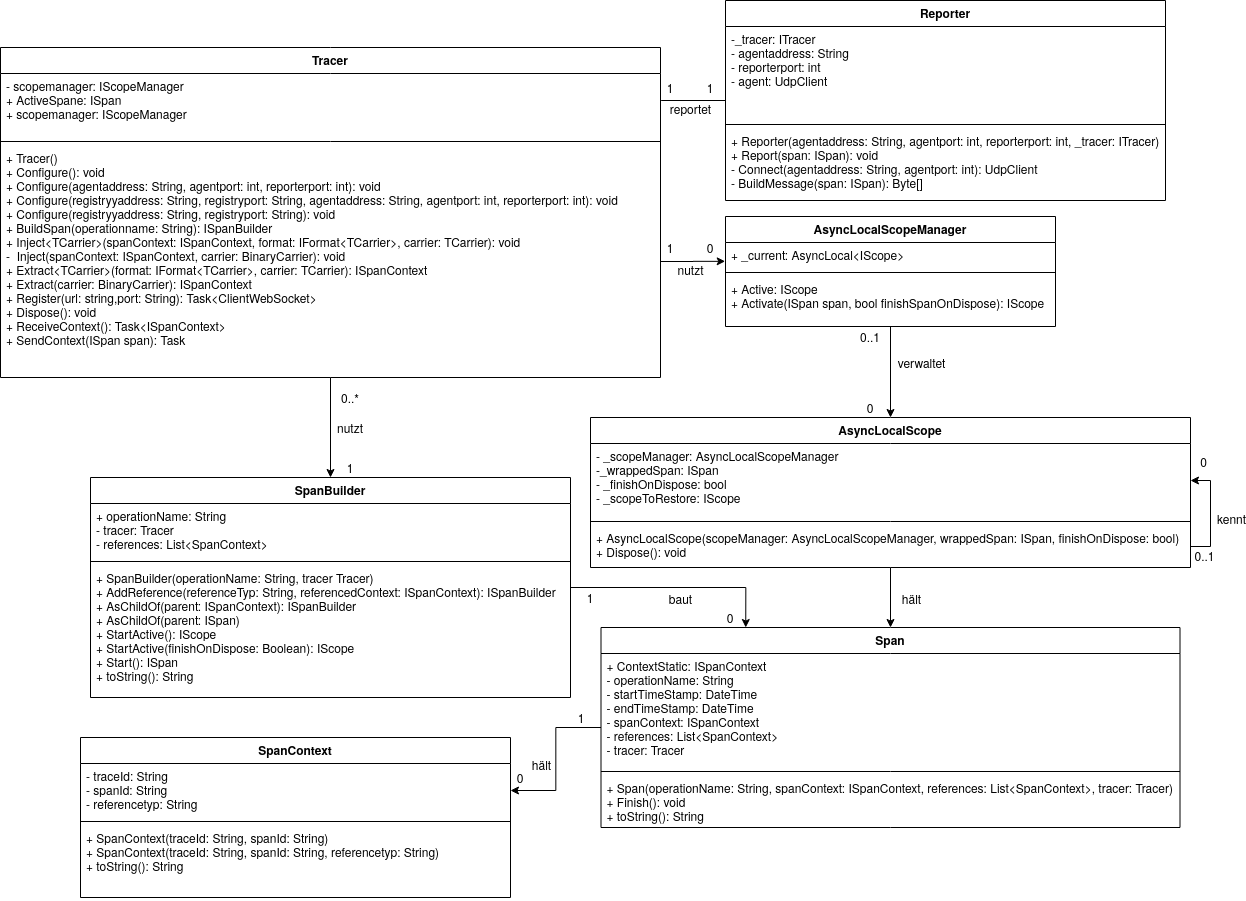
\includegraphics[scale=0.4]{img/Implementierung/TraktorKlassendiagramm.png}
		\caption[Klassendiagramm der Traktor Instrumentalisierungsbibliothek]{Klassendiagramm der Traktor Instrumentalisierungsbibliothek}
		\label{fig:TraktorKlassendiagramm}
	\end{figure}
\end{landscape}

\section{Traktor Agent}
\label{section:Traktor Agent}

Der Traktor Agent ist ein Service, welcher einen \gls{udpLabel}-Endpunkt bereitstellt. Der Service gibt alle erhaltenen Nachrichten auf seiner Konsole aus. Zwei Umgebungsvariablen werden genutzt, um den \gls{udpLabel}-Endpunkt zu initialisieren. Die \textbf{UDP\_IP} ist der \emph{Localhost}, da der Service auf einer eigenständigen Komponenten bereitgestellt wird. Dies ist durch den Spezifikikationspunkt \textbf{TE}.2  gegeben. Der belegete Port wird durch die Umgebungsvariable \textbf{UDP\_PORT} konfiguriert. 

Ein reporteter Span kann folgendermaßen aussehen:

\begin{minipage}[]{\textwidth}
	\begin{lstlisting}[frame=trBL]
	traktor-agent_1| recieved message: 
		 b'Process Context;
		 04/14/2020 10:10:06.1791 PM;
		 WIoJiNwldhLM;ZtDdH4lQ1a1b;
		 child_of;
		 04/14/2020 10:10:06.4158 PM'
	traktor-agent_1| from:  ('172.22.0.5', 13338)
	\end{lstlisting}
	\captionof{lstlisting}{Ein reporteter Span. Der gezeigte Span ist in der Webserver Entwicklungsumgebung generiert worden}
	\label{listing:Reporteter-Span}
\end{minipage} 

Der Service \emph{traktor-agent\_1} erhält von der Netzwerkadresse 172.22.0.5:13338 die dargestellte Nachricht eines Spans mit dem Operationsnamen \emph{Process Context}. Der Startzeitstempel und der Endzeitstempel sind Teil des reporteten Spans. Auch der Spankontext ist dargestellt.

\section{Traktor Registry}
\label{section:Traktor Registry}

Die Traktor Registry ist ein Websocket Server. Verbindungsanfragen, initiiert von einer Tracerinstanz, werden als eigenständiger Thread in einer Klienten-liste der Registry gespeichert. Die Anwendungslogik der \emph{ClientHandler}-Threads implementiert die Websocket Handshakes. Das Websocketprotokoll wird in \cref{subsection:Websocketprotokoll} beschrieben. Die Kontextpropagierung wird durch den Websocket Server umgesetzt. Die Implementierung wird in \cref{subsection:Klientenverwaltung} vorgestellt.

\subsection{Websocketprotokoll}
\label{subsection:Websocketprotokoll}

Das Websocketprotokoll ermöglicht eine voll-duplex Kommunikation zwischen der Registry und dem entsprechenden Websocketklienten eines Tracers. Das Protokoll nutzt dafür eine einzige TCP-Verbindung. Das Websocketprotokoll wird genutzt, um einen geringen \textbf{Overhead} der Kommunikation zu gewährleisten. Dementsprechend wird das Designziel der \textbf{Verarbeitungskosten} berücksichtigt. Das Websocketprotokoll ist durch \gls{rfcLabel} mit der Nummer 6455 spezifiziert.

Das Websocketprotokoll verlangt einen öffnenden Handshake zur Etablierung der Verbindung. Dieser basiert auf einem HTTP Handshake. Die eröffnende HTTP-Anfrage beinhaltet eine \emph{Upgrade}-Anforderung, der in diesem Moment genutzten HTTP-Verbindung. Der folgende Ausschnitt eines Logs, zeigt eine solche Eröffnungsnachricht:

\begin{minipage}[]{\textwidth}
	\begin{lstlisting}[frame=trBL]
	GET / HTTP/1.1
	Host: traktor-registry:8090
	Connection: Upgrade
	Upgrade: websocket
	Sec-WebSocket-Version: 13
	Sec-WebSocket-Key: s4VKefPmikGz1rJ24buoaQ==
	\end{lstlisting}
	\captionof{lstlisting}{Eröffnende Nachricht eines Websocket Handshake}
	\label{listing:Eröffnender Websocket Handshake}
\end{minipage} 

Die HTTP-Nachricht beinhaltet sogenannte \textbf{Header}, die Daten beinhalten, die für den Protokollwechsel von HTTP zu Websocket nötig sind. Der Host-Header identifiziert den Ursprung des Handshakeinitiators. Dieser ist in diesem Falle die IP-Addresse die hinter dem Alias \emph{traktor-registry} steht. Der Port 8090 der Anwendung, von welchem die Anfrage stammt, wird zusätzlich mitgesendet. Der Connection-Header gibt die bevorzugte Verbindungsart an. Diese beschreibt den gewünschten Vorgang eines Upgrades der Verbindung. In Verbindung mit dem Inhalt des Connections-Headers wird ein Upgrade-Header gesendet. Dieser ist ein Vorschlag an den Server ein anderes Protokoll zu nutzen. Entsprechend beinhaltet der Upgrade-Header den Vorschlag das Websocket Protokoll zu verwenden. Die letzen beiden Header Sec-WebSocket-Version und Sec-WebSocket-Key sind websocketspezifische Header.

Die Serverantwort sieht ähnlich aus. Diese besteht aus der Request-Line und dem Sec-WebSocket-Accept Header, der eine Bestätigung der zu nutzenden Websocketverbindung darstellt.

\begin{minipage}[]{\textwidth}
	\begin{lstlisting}[frame=trBL]
	HTTP/1.1 101 Switching Protocols
	Upgrade: websocket
	Connection: Upgrade
	Sec-WebSocket-Accept: HSmrc0sMlYUkAGmm5OPpG2HaGWk=
	\end{lstlisting}
	\captionof{lstlisting}{Serverantwort eines Websocket Handshake}
	\label{listing:Serverantwort eines Websocket Handshake}
\end{minipage} 

Bei einem erfolgreichen Handshake bleibt die Verbindung kommunikationsbereit, bis der Tracer die Verbindung manuell schließt.

Die Implementierung des Websocket Servers basiert auf Grundlage eines Guides von Mozilla und wurde entsprechend den Implementierungsanforderungen angepasst und erweitert.\footpartcite{MozillaWebsocket} Nachfolgend wird die Implementierung der Antwort auf einen Websocketverbindungsanfrage gezeigt:

\begin{minipage}[]{\textwidth}
	\begin{lstlisting}[frame=trBL]
	string swk = Regex.Match(s, "Sec-WebSocket-Key: (.*)")
									.Groups[1].Value.Trim();
	string swka = swk + "258EAFA5-E914-47DA-95CA-C5AB0DC85B11";
	byte[] swkaSha1 = System.Security.Cryptography.SHA1.Create()
									.ComputeHash(Encoding.UTF8
									.GetBytes(swka));
	string swkaSha1Base64 = Convert.ToBase64String(swkaSha1);
	
	byte[] response = Encoding.UTF8.GetBytes(
									"HTTP/1.1 101 Switching Protocols\r\n" +
									"Connection: Upgrade\r\n" +
									"Upgrade: websocket\r\n" +
									"Sec-WebSocket-Accept: " + swkaSha1Base64 +
									"\r\n\r\n");
	
	stream.Write(response, 0, response.Length);
	\end{lstlisting}
	\captionof{lstlisting}{Implementierung der Serverantwort eines Websocket Handshake}
	\label{listing:Implementierung der Serverantwort eines Websocket Handshake}
\end{minipage}

Der Wert von \emph{Sec-WebSocket-Key} wird extrahiert und von führenden und folgenden Leerzeichen bereinigt. Anschließend wird der Wert mit einer speziellen \gls{guidLabel} konkateniert. Dieser zusammengesetzte String wird schließend mit SHA-1\footpartcite{fette2011websocket}, einem kryptographischen Hash Algorithmus, verschlüsselt. Der verschlüsselte Wert wird daraufhin mit Base64 kodiert, die Serverantwort gebaut und anschließend an den Tracerklienten gesendet.

Der Websocket Server muss in der Lage sein, auf eine Schließung der Websocketverbindung reagieren zu können. Dementsprechend muss eine Schließungsnachricht gebaut werden.
Diese Schließungsnachricht ist ein 2-Byte großer Frame. Die \cref{fig:WebsocketClosingFrame} visualisiert einen Websocketschließungs-Frame. Der Frame besteht aus einem FIN-Bit, der auf 1 gesetzt sein muss. RSV1, RSV2 und RSV3 sind reservierte Bits, die auf 0 gesetzt sein müssen. Der Opcode ist ein 4-Bit großer Flag, der dem Dezimalwert 8 entspricht. Dieser steht für die Operation des Schließens des Websockets. Die Maske ist auf 0 gesetzt. Auch sind die Bits der Payload Length auf 0 gesetzt. 

\begin{figure}[!ht]
	\centering
	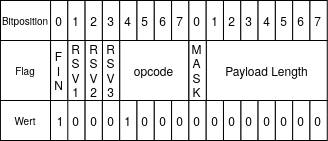
\includegraphics[scale=0.8]{img/Implementierung/WebsocketClosingFrame.png}
	\caption[Websocket Closing Frame]{Websocket Closing Frame}
	\label{fig:WebsocketClosingFrame}
\end{figure}


\subsection{Klientenverwaltung}
\label{subsection:Klientenverwaltung}

Bei erfolgreich hergestellter Websocketverbindung, kann die Registry auf Kontextpropagierung reagieren. 
Die Klienten werden in einem seperaten Thread behandelt. 
Ein Thread beinhaltet jeweils einen Datenstrom. 
Der Thread implementiert eine Dauerschleife. 
In dieser Dauerschleife wird der Datenstrom kontinuierlich überprüft. 
Bei eingehenden Daten wird überprüft, um welchen Datentypen es sich handelt. 
Dieser Prozess ist zum Teil in dem Aktivitätsdiagramm, gezeigt in \cref{fig:Traktor-Registry}, visualisiert.
Es werden drei Nachrichtentypen unterschieden:
\begin{itemize}
	\item Tracerklient Anmeldung
	\item Tracerklient Abmeldung
	\item Kontextübermittlung
\end{itemize}

Der Nachrichtentyp der Anmeldung, lässt sich anhand der Request-Line feststellen. 
Bei Abmeldungen und Nachrichten, die Kontextübermittlung einleiten sollen, kann dies durch den \emph{opcode} festgestellt werden.
Die Implementierungsdetails der An- und Abmeldung wurde in \cref{subsection:Websocketprotokoll} ausgeführt. 
Im Falle der Kontextübermittlung wird die Nachricht zuerst decodiert. 
Da die Nachricht von einem Websocketklienten stammt, ist der \textbf{Mask} bit gesetzt. 
Dies ist in \gls{rfcLabel} 6455 spezifiziert. 
Dementsprechend muss die Nachricht umformatiert werden, damit sie weiterverarbeitet werden kann. Die Nachricht wird im Registry-Log ausgegeben und anschließend wird der Kontext an alle Teilnehmenden Tracerklienten versendet. In der Implementierung ist noch keine Addressierung der Kontextnachrichten umgesetzt. Das bedeutet, dass alle teilnehmenden Klienten die Kontextnachricht empfangen, abgesehen von dem Klienten, der die Nachricht versendet hat. Dies kann in Systemen mit mehr als zwei Tracerinstanzen zu Komplikationen mit dem Nachrichtenstrom führen, da abgesehen von dem Zieltracer des Kontext, keine Kontextnachrichten erwartet werden.

\section{Traktor Interceptor}
\label{section:Traktor Interceptor}
Der Traktor Interceptor dient als Alternativkonzept zu der Traktor Registry. Der Traktor Interceptor setzt eine Nachrichtenmodifikation um, bei der die Nachrichten, die durch die Betriebssystemnetzwerksinterfaces geleitet werden, abgefangen und erweitert werden. Bei dem Eintreffen der Nachricht in der Empfängerkomponente wird die Nachricht abermals abgefangen und die Metadaten extrahiert. Der Traktor Interceptor wird als Python Script umgesetzt. Auf jeder Komponente des Systems muss dieses Script während der Laufzeit der instrumentalisierten Anwendung ausgeführt werden. Der implementierte Prototyp soll als \emph{Proof of Concept} dienen. Das Abhören der Netzwerkschnittstelle und das Manipulieren der Pakete ist mithilfe der Paketmanipulationsbibliothek Scapy umgesetzt. Das Script beinhaltet eine Schleife, bei der bei eintreffender Websocketnachricht eine Callback Funktion aufgerufen wird. Die Callback Funktion erhält als Parameter die Nachricht. Es wird untersucht, ob die Nachricht den Spezifikationen eine Websocketnachricht entspricht. Anschließend wird die Nachricht in ihre Komponenten zerlegt, wieder zusammengebaut und an ihren Empfänger weitergeleitet. Der Prototyp zeigt, dass eine Paketmanipulation möglich ist.

\section{Unity Rendering-System}
\label{section:Unity Rendering System}

Das verteilte Rendering-System dient zur Generierung von Frames auf Grundlage von dreidimensionalen Geodaten. Dabei wird ein Ansatz verwendet, um die Vorteile einer verteilten Anwendung zu nutzen. Das heißt, dass viele Komponenten des Systems Teilaufgaben bearbeiten. Die Arbeit, die von den Komponenten verrichtet wird, ist das Generierung von Teilframes. Die Teilframes werden in einem Kollektor zusammengeführt und anschließend an den anfragenden Klienten gesendet. Die Anwendung verwendet die Unity Engine als Renderer. Die Instrumentalisierung findet innerhalb der Scripts statt, die für den Renderprozess ausgeführt werden. In dem verteilten Rendering-System ist das Event des Generierens und des Absendens eines Frames von Interesse. Dieses Event wird von der Instrumentalisierungsbibliothek als Traces dargestellt.
Dadurch wird die Zeit aufgezeichnet, die für die Generierung eines Frames benötigt wird. Aufgrund der Struktur des Projekts, lassen sich keine detaillierteren Events, wie z.B. das Empfangen der Klientenanfrage oder das Senden des Frames, darstellen. 

Die Instrumentalisierung ist durch das Hinzufügen eines Scripts und der Modifikation eines bestehenden realisiert.
Das hinzugefügte Script \emph{LoggingServerSideRendering} beinhaltet eine Klasse, dessen Objekt als Tracer innerhalb eines Scripts genutzt werden kann.
Aufgrund der hoch asynchronen und parallelen Natur der Appliktion ist es notwendig eine dynamische Portermittlung für den Reporter zu ermöglichen.
Dazu wurde ein Portbereich bekanntgegeben, in dem ein freier Port ausgewählt wird.
Jeder parallele Prozess, der einen Tracer nutzt, wartet auf die Beendigung des Konfigurationsprozesses des Tracers.
Dies hat zur Folge, dass die Prozesse auf den Tracer warten müssen.
Das widerspricht dem Designziel der Verarbeitungskosten. Dieser Umstand ist jedoch als Kompromiss zu sehen. Der Kompromiss besteht darin, die Nutzung des Tracers innerhalb der Unity Anwendung möglichst benutzerfreundlich zu machen, also dem Designziel der Benutzbarkeit zu entsprechen.

Die Instrumentalisierung befindet sich in der \emph{GBufferSource} Klasse.
Die Klasse umfasst den Renderingvorgang eines Frames. 
Dieser Vorgang wird als ein zu verfolgendes Event bestimmt.
In \cref{listing:Instrumentalisierung der GBufferSource Klasse} ist der Codeabschnitt dargestellt, der instrumentalisiert ist.
Die Instrumentalisierung umfasst das Rendern, durchgeführt durch ein \emph{\_camera} Objekt und die Frameextraktions aus dem nativen Plugin.


\begin{minipage}[]{\textwidth}
	\begin{lstlisting}[frame=trBL]
	using (var scope = LoggingServerSideRendering.Tracer
					.BuildSpan("Render Frame")
					.StartActive(true))
	{
				_camera.Render();
				_nativeGBufferExtraction.NewFrameRendered(Time.frameCount);
	}
	
	\end{lstlisting}
	\captionof{lstlisting}{Instrumentalisierung der GBufferSource Klasse}
	\label{listing:Instrumentalisierung der GBufferSource Klasse}
\end{minipage}

\section{ Webserver Entwicklungsumgebung }
\label{section:Webserver Entwicklungsumgebung}

In diesem Kapitel wird die Traktorentwicklungsumgebung vorgestellt. Diese Testumgebung gewährleistet, dass die Funktionalitäten der Instrumentalisierungsbibliothek in einer Beispielanwendung angewandt werden können. Das System besteht aus vier Komponenten. Eine Übersicht der Komponenten ist in der \cref{fig:TraktorEnv-ApplicationArchitecture} gezeigt. Neben der bereits beschriebenen Traktor Registry und dem Traktor Agent, werden zwei Webserver eingeführt. Die beiden C\# Webserver \emph{Traktor-Fibonacci-Caller} und \emph{Traktor-Fibonacci-Server} sind mit Traktor instrumentalisiert. Sie dienen dazu, einen Nachrichtenaustausch zu ermöglichen, der sich durch das ganze System zieht. Die Applikation ermöglicht es einem Anwender, eine Zahl der Fibonacci-Folge zu berechnen. Die Nachricht die der Anwender an den Traktor-Fibonacci-Caller-Service sendet, beinhaltet im \emph{Body} eine Zahl mit dem Variablennamen N. Die Zahl repräsentiert die zu berechnende Stelle der Fibonacci-Folge. In \cref{listing:Implementierung der Serverantwort eines Websocket Handshake} wird eine beispielhafte Anfrage gezeigt. Es wurde sich für die Implementierung eines simplen und rekursiv anwendbaren Algorithmus entschieden, da die Testumgebung nicht durch die Anwendungslogik der Webserver verkompliziert werden sollte. Ausserdem ermöglich die Rekursivität des Algorithmus, eine schnell zu skalierende Anzahl an generierten Events, mit einem deutlich erkennbaren und messbaren zeitlichen Unterschied. Die Grundstruktur der beiden Webserverimplemetierungen ist gleich. Ein C\# Programm startet ein Serverobjekt, welcher einen Thread beinhaltet, der eine API bereitstellt, die über HTTP ansprechbar ist. Nachfolgend wird auf die Instrumentalisierung der Webserver eingegangen.

\begin{minipage}[]{\textwidth}
	\begin{lstlisting}[frame=trBL]
	PUT / HTTP/1.1
	Accept: application/json, */*
	Accept-Encoding: gzip, deflate
	Connection: keep-alive
	Content-Length: 8
	Content-Type: application/json
	Host: 172.22.0.5:8085
	User-Agent: HTTPie/0.9.8
	
	{
	"N": 3
	}
	\end{lstlisting}
	\captionof{lstlisting}{HTTP-Anfrage an den Traktor-Fibonacci-Caller durch den HTTP-Klient HTTPie}
	\label{listing:Implementierung der Serverantwort eines Websocket Handshake}
\end{minipage}


\textbf{Traktor-Fibonacci-Caller}\space\space\space Sowohl der Traktor-Fibonacci-Caller als auch der Traktor-Fibonacci-Server basieren auf dem gleichen Aufbau. Beim Starten der Anwendung wird, abhängig von der Betriebssystemfamilie, die Tracerkonfiguration durchgeführt. 
Auf einem Unix-basierenden Betriebssystem, wird die Konfiguration über Umgebungsvariablen gehandhabt. 
Da der Server einen Tracer beinhaltet, sind die für die Registry-Verbindung benötigten Umgebungsvariablen zu setzten. 
Diese sind die \emph{REGISTRY\_IP} und der \emph{REGISTRY\_PORT}. 
Für die Verbindung zum Traktor-Agenten werden die entsprechenden Umgebungsvariablen \emph{AGENT\_IP} und \emph{AGENT\_PORT} erwartet.
Für den einzunehmenden Port des Tracers, über den die reporteten Spans zum Agenten gesendet werden, wird der \emph{REPORTER\_PORT} zur Konfiguration genutzt. 
Der Server ist nach seiner Initialisierung einsatzbereit und erwartet Nachrichten. 
Sobald eine Nachricht eintrifft, wird die \emph{Proccess} Funktion aufgerufen. 
Die Process Funktion erhält einen HTTP Kontext als Paramenter. 
Dieser beinhaltet die Nutzdaten des Anwenders, die mittels HTTP-Klienten gesendet wurden.

Der instrumentalisierte Codeabschnitt des Callers ist folgendermaßen implementiert:

\begin{minipage}[]{\textwidth}
	\begin{lstlisting}[frame=trBL]
	private void Process(HttpListenerContext context){
		using (var scope = Program.tracer.BuildSpan("Process Context")
						.StartActive())
		{
			var body = new StreamReader(context.Request.InputStream, Encoding.UTF8)
						.ReadToEnd();       
			var json = JsonSerializer.Deserialize<JsonObject>(body);
			Program.tracer.SendContext(scope.Span).GetAwaiter().GetResult();
			string response = SendRequest(fibo_ip,fibo_port,json);
			context = BuildResponse(context, response);
			context.Response.Close();
		}
	}
	\end{lstlisting}
	\captionof{lstlisting}{Process Funktion des Fibonacci-Caller Services}
	\label{listing:Process Funktion des Fibonacci-Caller Services}
\end{minipage}

Das \emph{using} Statement dient zum automatischen Schließen, der in ihr genutzten Ressource. 
Dies ist in diesem Fall das Scope Objekt. 
Der Tracer baut einen neuen Span mit dem Operationsnamen \emph{Process Context} und makiert in als aktiv. 
Die Nutzdaten werden aus der HTTP-Nachricht extrahiert. 
Die aktuell als JSON-Objekt vorliegenden Daten, werden deserialisiert. 
Da der Tracerkontextwechsel bevorsteht, wird der Kontext des Spans an die Registry, mittels \emph{SendContext}, gesendet und auf einen erfolgreichen Abschluss gewartet. 
Es ist zu diesem Zeitpunkt davon auszugehen, dass der Zieltracer bereit ist, den empfangen Kontext zu verarbeiten. 
Aus diesem Grund werden die Nutzdaten an den Trakor-Fibonacci-Server im JSON-Format als weiterer Request gesendet. 
Sobald das Ergebnis vom Fibonacci Server eintrifft, wird die Antwort, welcher zum HTTP-Klienten zurückkehrt, gebaut und übermittelt. 
Aufgrund des using-Statements beendet die Lebensspanne des Scope Objekts und der Span wird an den Traktor-Agent reportet. 

\textbf{Traktor-Fibonacci-Server}\space\space\space Der Fibonacci-Server beinhaltet den Algorithmus zur Berechnung der Fibonaccizahl. 
Innerhalb des Server sind zwei Funktionen instrumentalisiert. Dies ist zum einen, wie auch im Fibonacci-Caller, die \emph{Process} Funktion, aufgeführt in \cref{listing:Process Funktion des Fibonacci-Server Services}. 
Die Funktion zeigt das Empfangen des Tracingkontexts durch den Aufruf der Funktion \emph{ReceiveContext}. Ein neuer Span wird manuell erstellt. 
Die Relation wird durch die Tracerfunktionalität \emph{AsChildOf(parentContext)} hergestellt. 
Anschließend wird der Span gestartet und aktiviert. 
Die Nutzdaten werden extrahiert und die zweite instrumentalisierte Funktion \emph{CalculateFibonacci} wird aufgerufen. 

\begin{minipage}[]{\textwidth}
	\begin{lstlisting}[frame=trBL]
	private async void Process(HttpListenerContext context)
	{
		ISpanContext parentContext = await Program.tracer
							.ReceiveContext();
		string response;
		var span = Program.tracer.BuildSpan("Server: Process Context")
							.AsChildOf(parentContext)
							.Start();
		Program.tracer.ScopeManager.Activate(span,true);
		var body = new StreamReader(context.Request.InputStream, Encoding.UTF8)
							.ReadToEnd();       
		var json = JsonSerializer.Deserialize<JsonObject>(body);
		response = CalculateFiboncacci(json.N).ToString();
		response = "result=" + response;
		byte[] b = Encoding.UTF8.GetBytes(response);
		[...]
		context.Response.Close();
		span.Finish();
	}
	\end{lstlisting}
	\captionof{lstlisting}{Process Funktion des Fibonacci-Server Services}
	\label{listing:Process Funktion des Fibonacci-Server Services}
\end{minipage}

Die CalculateFibonacci Funktion ist bewusst rekursiv und möglichst ineffizient implementiert. Die Funktion braucht zur Berechnung des $n$te Elements $(2 * Fn) - 1$ rekursive Aufrufe, wobei $Fn$ die ermittelte Fibonaccizahl ist. Dadurch ist es möglich, einen großen Trace zu erzeugen. Die Funktion nutzt das using-Statement, um beim Beenden des Codeabschnitt den Span automatisch zu reporten. \emph{CalculateFibonacci} ist als Operationsname gegeben.

\begin{minipage}[]{\textwidth}
	\begin{lstlisting}[frame=trBL]
	private int CalculateFiboncacci(int n) 
	{
		using (var scope = Program.tracer.BuildSpan("CalculateFiboncacci")
						.StartActive())
		{
			if (n == 0) return 0;
			else if (n == 1) return 1;
			return  ( CalculateFiboncacci(n - 1) + CalculateFiboncacci(n - 2) );
		}
	}
	\end{lstlisting}
	\captionof{lstlisting}{Instrumentalisierte CalculateFibonacci Funktion des Fibonacci-Server Services}
	\label{listing:Instrumentalisierte CalculateFibonacci Funktion des Fibonacci-Server Services}
\end{minipage}

\cref{fig:TraktorEnv-ApplicationArchitecture} bietet eine Architekturübersicht. Es werden die Kommunikationswege, sowie die Services dargestellt, die implementiert und beschrieben wurden.

\begin{figure}[]
	\centering
	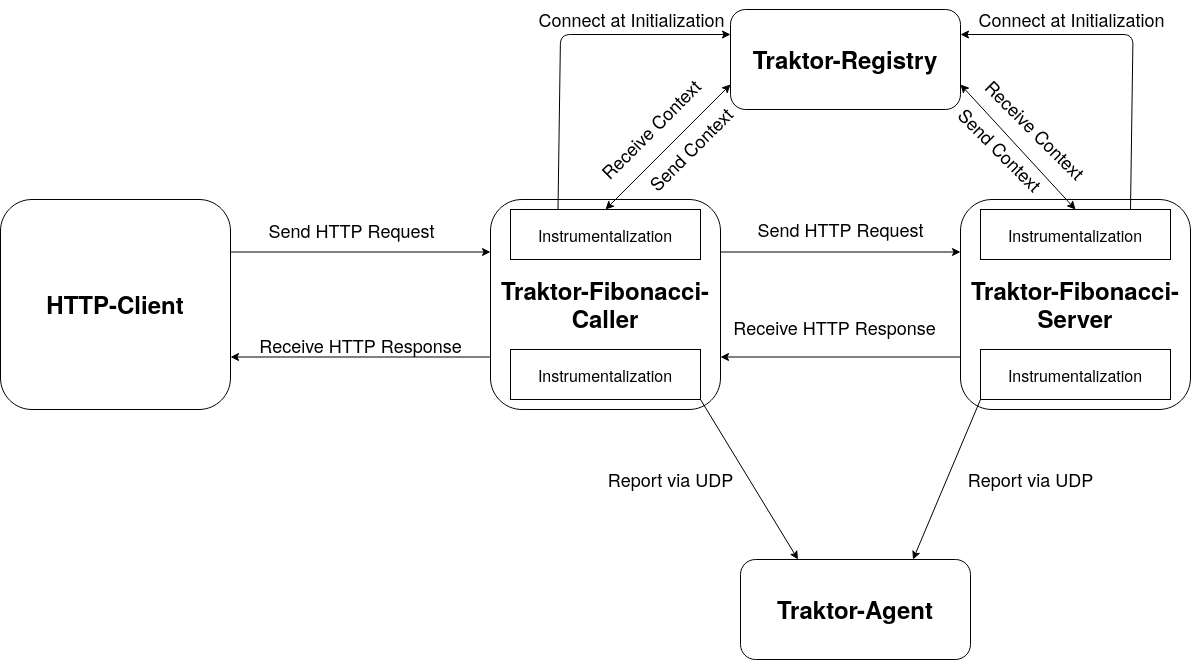
\includegraphics[scale=0.3]{img/Implementierung/TraktorEnv-ApplicationArchitecture.png}
	\caption[Systemübersicht der Traktorentwicklungsumgebung]{Systemübersicht der Traktorentwicklungsumgebung}
	\label{fig:TraktorEnv-ApplicationArchitecture}
\end{figure}
% ----------------------------------------------------------------------------

% ----------------------------------------------------------------------------
% Copyright (c) 2016 by Burkhardt Renz. All rights reserved.
% Die Vorlage für eine Abschlussarbeit in der Informatik am Fachbereich
% MNI der THM ist lizenziert unter einer Creative Commons
% Namensnennung-Nicht kommerziell 4.0 International Lizenz.
%
% Id:$
% ----------------------------------------------------------------------------

\chapter{Evaluierung}
\label{chapter:Evaluierung}
In diesem Kapitel werden die Prozesse beschrieben, die durchgeführt wurden, um die Implementierung und die erhaltenen Ergebnisse zu evaluieren. In \cref{section:Anforderungserfüllung} wird die Traktorimplementierung auf ihre Einhaltung der Anforderungen  untersucht. In \cref{section:Umsetzung der Designziele} werden die Designziele herangezogen und auf ihre Gegebenheit in der Tracingbibliothek überprüft. Das Open-Source Projekt \textbf{Jaeger} wird als Vergleichswerkzeug in den Folgenden Abschnitten herangezogen. Jaeger ist eine auf der OpenTracing API basierenden \emph{state-of-the-art} Distributed Tracing Implementierung. Sie setzt die aktuellsten Erkenntnisse der Distributed Tracing Gemeinschaft um. Dabei wird in \cref{section:Bereitstellung der Testumgebung} die Bereitstellung der Testumgebung, in Hinsicht auf beide Werkzeuge, diskutiert. Die Bereitstellungsunterschiede beider Werkzeuge werden aufgezeigt. In \cref{section:Ergebnissvergleich} werden die Ergebnisse der Spangenerierung verglichen. Es wird auf die Ausdruckskraft des Traktor-Datenmodells im Vergleich zu Jaeger eingegangen. Zuletzt werden die präsentierten Visualisierungansätze diskutiert. Es wird ein Vergleich zu den Visualisierungsmöglichkeiten der Jaeger UI durchgeführt.

\section{Anforderungserfüllung}
\label{section:Anforderungserfüllung}

Es ist eine Analyse durchzuführen, bei der die erhobenen Daten interpretiert werden. Die daraus gewonnenen Informationen sollen die End-zu-End Latenz einer Anfrage durch ein verteiltes System und die Generierungszeit eines Frames, welches durch die Unity Anwendung generiert wurde, darstellen. 

Die Implementierungsphase erfolgte nach dem Softwareentwicklungskonzept des \gls{tddGlossar}. Test-driven development ist ein Software Entwicklungskonzept, dass darauf basiert, kurze Iterationsphase, durch die Implementierung von Tests und anschließender Funktionalitätsumsetzung, durchzuführen. Die Tests sollen den Anforderungen entsprechen, die an die Funktion gestellt werden. Die Mitentwicklung der Testbasis ermöglicht eine sich stetig verbessernde Rückmeldung der Codequalität. Auch eine anschließende Projektbereitstellungsautomatisierung wird damit erleichtert. Es wird also verhindert, dass sich technisch Schulden anhäufen.

Die Anforderungen der Funktionalitäten ist anhand der Implementierungen und der Tests gegeben. Ein Beispieltest vermittelt den Aufbau der Tests.

\begin{minipage}[]{\textwidth}
	\begin{lstlisting}[frame=trBL]
	[TestMethod]
	public void StartActive()
	{
	string expectedOperationName = "Testoperation";
	Tracer tracer = new Tracer();
	ISpanBuilder builder = tracer.BuildSpan(expectedOperationName);
	IScope scope = builder.StartActive();
	string[] actualSpanFields = scope.Span.ToString().Split(";");
	
	Assert.AreEqual(scope.Span, tracer.ActiveSpan);
	Assert.AreEqual(scope.Span, tracer.ScopeManager.Active.Span);
	Assert.AreEqual(tracer.ActiveSpan, tracer.ScopeManager.Active.Span);
	}
	\end{lstlisting}
	\captionof{lstlisting}{Unit-Test der Spanbuilder Klasse}
	\label{listing:Unit-Test der Spanbuilder Klasse}
\end{minipage}

Der StartActive Test, testet die Funktion \emph{StartActive} der SpanBuilder Klasse. Dabei wird eine Operationsname ein Scope initialisiert, der einen Span beinhaltet. Der Span wird aktiviert und mit dem Span verglichen, der in dem Scopemanager verwaltet wird. Bei übereinstimmenden Werten der Felder, ist der Test bestanden und die Funktion entspricht den Anforderungen, die an diese gestellt werden.

Die Anforderung der End-zu-End Latenz und die Anforderung an der Bestimmung der Generierungszeit eines Frames werden durch das Datenmodell erfüllt. Durch die Führung von \emph{Datetime} Objekten innerhalb der Spans, lassen sich Zeitspannen bestimmen, die ein Event einnimmt. Die Differenz aus Endzeit und Startzeit ergibt die Zeitspanne der Framegenerierung, da der Prozess der Framegenierung durch einen Span darstellbar ist. Die End-zu-End Latenz ergibt sich aus dem hierarchisch am höchsten angeordneten Span eines Traces und den darüber hinaus, falls vorhanden, folgenden Spans, die den Beziehungstypen \emph{follows-from} besitzen. Die Differenz der Startzeit des ersten Spans und der Endzeit des letzten Spans ergibt die End-zu-End Latenz, die durch die Anfrage entsteht.

Die Rahmenbedingung der eingeschränkten Nachrichtenmodifikation ist durch die Umsetzung des Konzept der Kontextpropagierung mittels dem Registry Service eingehalten. Die Kommunikationswege der Anwendungen werden dadurch nicht beansprucht.


\section{Umsetzung der Designziele}
\label{section:Umsetzung der Designziele}
\begin{itemize}
	\item Durch Docker-Compose wird eine verteiltes System auf einem Lokalen Rechner aufgebaut.
	\item gibt es architektonische unterschiede? Services etc. 
	\item Konfigurationsunterschiede
	\item Ist traktor einfacher zu deployen? Wahrschienlich nicht da jaeger ein all in one image hat. Könnte aber auch umgesetzt werden
\end{itemize}

\section{Bereitstellung der Testumgebung}
\label{section:Bereitstellung der Testumgebung}

\section{Ergebnissvergleich}
\label{section:Ergebnissvergleich}
Die Dateninterpretation wird auf Basis eines Datensatzes durchgeführt, welche aus der Traktorentwicklungsumgebung erhoben worden sind. 

Die Rohdaten sehen folgendermaßen aus:

\begin{minipage}[]{\textwidth}
	\begin{lstlisting}[frame=trBL]
	recieved message:  b'Server: Process Context;04/22/2020 09:29:00.1081 PM;S17JnBOXEmes;rtXWWLvE9XDg;child_of;04/22/2020 09:29:00.1097 PM{pi1a+hw7UuZN:child_of}'
	from:  ('172.22.0.5', 13337)
	recieved message:  b'CalculateFiboncacci;04/22/2020 09:29:00.1083 PM;S17JnBOXEmes;8glMa3Uu+jy2;child_of;04/22/2020 09:29:00.1084 PM{75buv+V8lmUn:child_of}'
	from:  ('172.22.0.5', 13337)
	recieved message:  b'CalculateFiboncacci;04/22/2020 09:29:00.1086 PM;S17JnBOXEmes;8V4vMLWZ2Ax/;child_of;04/22/2020 09:29:00.1086 PM{75buv+V8lmUn:child_of}'
	from:  ('172.22.0.5', 13337)
	recieved message:  b'CalculateFiboncacci;04/22/2020 09:29:00.1083 PM;S17JnBOXEmes;75buv+V8lmUn;child_of;04/22/2020 09:29:00.1087 PM{wngEpk/UsI3i:child_of}'
	from:  ('172.22.0.5', 13337)
	recieved message:  b'CalculateFiboncacci;04/22/2020 09:29:00.1089 PM;S17JnBOXEmes;wJ5dqhRUsV8h;child_of;04/22/2020 09:29:00.1089 PM{wngEpk/UsI3i:child_of}'
	from:  ('172.22.0.5', 13337)
	recieved message:  b'CalculateFiboncacci;04/22/2020 09:29:00.1083 PM;S17JnBOXEmes;wngEpk/UsI3i;child_of;04/22/2020 09:29:00.1090 PM{rtXWWLvE9XDg:child_of}'
	from:  ('172.22.0.5', 13337)
	recieved message:  b'Process Context;04/22/2020 09:29:00.0948 PM;S17JnBOXEmes;pi1a+hw7UuZN;child_of;04/22/2020 09:29:00.1188 PM'
	from:  ('172.22.0.4', 13338)
	\end{lstlisting}
	\captionof{lstlisting}{Tracerrohdaten aus der Traktorentwicklungsumgebung}
	\label{listing:Tracerrohdaten aus der Traktorentwicklungsumgebung}
\end{minipage}

Diese Rohdaten sind in dem Agenten eingetroffen, nachdem sie von den beiden Tracer reportet worden sind. Anhand der \cref{fig:TraktorEnv-ApplicationArchitecture} .........

\begin{itemize}
	\item Bezug zur Problemstellung schaffen
	\item inwiefern hält sich jaeger an die Happens before relationship?
	\item wie setzt jaeger diese um?
	\item setzt es sie um?
	\item setzt traktor sie um? Wenn ja wie?
	\item Wie regelt Jaeger die Zeitresolution?
	\item  
\end{itemize}
\section{Visualisierungvergleich von Traktor und Jaeger}
\label{section:Visualisierungvergleich von Traktor und Jaeger}
\begin{itemize}
	\item jaeger bietet verschiedene visualisierungsmöglichkeiten
	\begin{itemize}
		\item z.B. DAG
		\item Tracediagramm
		\item Service-Orientierter Ansatz?
		\item Tracecompare
	\end{itemize}
	\item Welche Vorteile bringen meine Visualisierungsansatze?
	
\end{itemize}
% ----------------------------------------------------------------------------

% ----------------------------------------------------------------------------
% Copyright (c) 2016 by Burkhardt Renz. All rights reserved.
% Die Vorlage für eine Abschlussarbeit in der Informatik am Fachbereich
% MNI der THM ist lizenziert unter einer Creative Commons
% Namensnennung-Nicht kommerziell 4.0 International Lizenz.
%
% Id:$
% ----------------------------------------------------------------------------

\chapter{Fazit}
Die Hypothese, die in der Zielsetzung definiert worden ist, besagt, dass die Implementierungen der Inversenberechnung in C bessere Laufzeiten aufweisen, als in R.

Dies kann in Anbetracht der Messergebnis nur Teilweise bestätigt werden. 
\begin{itemize}
	\item Bei kleinen Matrizen trifft dies definitiv zu, wie in der Ergebnissdiskussion aufgezeigt wurde.
	\item Bei immer größer werdenden Matrizen steigt die Performance von R im Verhältnis zu den C-Varianten.
\end{itemize}

Diese Arbeit hat jedoch auch deutlich gemacht, wie stark die Performance von einer Implementierung abhängt. Es wurden gleiche Algorithmen mit unterschiedlichen Implementierungen verglichen und es hat sich herausgestellt, dass deutliche Unterschiede festzustellen sind. 

Die beiden naiven Ansätze leiden an gefährlichen Fehlern, wie z.B. Speicherlecks, die zum Absturz des Programms führen können. Das bedeutet, dass man bei der Auswahl seiner Werkzeuge, unbedingt die Rahmenbedingungen miteinbeziehen sollte. Damit ist gemeint, dass falls man die Möglichkeit hat, bewährte Packete einzusetzten, dann ist es empfohlen dies zu tun, anstatt das Rad neu zu erfinden.

Die C-Varianten können vorallem bei dem Speicherbedarf glänzen. Dafür sind jedoch hoher Entwicklungsaufwand und extreme Vorsicht bei der Implementierung aufzubringen.

Die R-Variante bietet eine enorme Auswahl an mathematischen Funktionen, die meistens sehr perfomant sind. Der Entwicklungsaufwand von Code ist ungemein geringer.

In Anbetracht der heutigen Ressourcen kann man in vielen Anwendungsfällen beruhigt auf die einfacheren Scriptsprachen zurückgreifen. Es lässt sich aber in speziellen Fällen nicht umgehen, die volle Kontrolle, bei z.B. sicherheitskritischen Bereichen, zu übernehmen. In diesem Fall bietet sich C an.
% ----------------------------------------------------------------------------

\backmatter 

\appendix
% ----------------------------------------------------------------------------
% Copyright (c) 2016 by Burkhardt Renz. All rights reserved.
% Die Vorlage für eine Abschlussarbeit in der Informatik am Fachbereich
% MNI der THM ist lizenziert unter einer Creative Commons
% Namensnennung-Nicht kommerziell 4.0 International Lizenz.
%
% Id:$
% ----------------------------------------------------------------------------


%\begin{thebibliography}{99}
\printglossary[type=main,title={Glossar}]
\printglossary[type=\acronymtype,title={Abkürzungsverzeichnis}]
%\end{thebibliography}

% ----------------------------------------------------------------------------



\end{document}
% ----------------------------------------------------------------------------
